%% ============================================================
%%  Physics-Informed Neural Networks and Quantum Dot Systems
%%  Author: Morten Hjorth-Jensen
%% ============================================================
%% graphicx is loaded by Beamer; real figure files are now linked.
\documentclass[aspectratio=169,10pt]{beamer}

%% ── Theme & colour ──────────────────────────────────────────────────────────
\usetheme{Madrid}
\usecolortheme{seahorse}
\usefonttheme[onlymath]{serif}

\setbeamercolor{frametitle}{bg=blue!15!white,fg=blue!60!black}
\setbeamercolor{title}{fg=blue!70!black}
\setbeamercolor{block title}{bg=blue!20!white,fg=blue!60!black}
\setbeamercolor{block body}{bg=blue!5!white}
\setbeamercolor{alerted text}{fg=red!60!black}
\setbeamertemplate{navigation symbols}{}

%% ── Packages ────────────────────────────────────────────────────────────────
\usepackage{amsmath,amssymb,bm,physics}
\usepackage{graphicx}
\usepackage{booktabs}
\usepackage{xcolor}
\usepackage{tikz}
\usepackage{makecell}
\usepackage[flushleft]{threeparttable}

%% ── Metadata ────────────────────────────────────────────────────────────────
\title[PINNs and Quantum Dots]{Physics-Informed Neural Networks\\
  and Properties of Quantum Dot Systems}
\author[M.~Hjorth-Jensen]{Morten Hjorth-Jensen}
\institute[UiO]{Department of Physics \& Center for Computing in Science Education\\
  University of Oslo, Norway}
\date{ECT* workshop on the Fermion sign Problem, Trento, April 20-24, 2026}

%% ============================================================
\begin{document}
%% ============================================================

%% ─── Slide 1: Title ─────────────────────────────────────────────────────────
\begin{frame}
  \titlepage
\end{frame}

%% ─── Slide 2: Outline ───────────────────────────────────────────────────────
\begin{frame}{Outline}
  \tableofcontents[hidesubsections]
\end{frame}

%% ============================================================
\section{Motivation and Context}
%% ============================================================

\begin{frame}{Quantum Dots as Artificial Atoms}
  \begin{columns}[T]
    \column{0.58\textwidth}
      \begin{itemize}
        \item Semiconductor quantum dots $\equiv$ \alert{artificial atoms}
        \item Precise tunability: particle number $N$, confinement $\omega$,
              interaction strength, external fields
        \item Intersection of condensed matter, quantum information
              and nanotechnology
        \item Rich many-body physics even for few particles:
          \begin{itemize}
            \item Wigner molecule formation
            \item Spin ordering
            \item Non-trivial excitation spectra
          \end{itemize}
        \item Clean realization of interacting fermions in reduced dimensions:
              Coulomb, exchange, quantum confinement all play essential roles
      \end{itemize}
    \column{0.38\textwidth}
      \begin{block}{Key parameters}
        \begin{tabular}{ll}
          $N$       & particle number \\
          $\omega$  & trap frequency  \\
          $\lambda$ & interaction strength
        \end{tabular}
      \end{block}
      \vspace{0.4cm}
      \begin{alertblock}{Core challenge}
        Hilbert space grows combinatorially with $N$
      \end{alertblock}
  \end{columns}
\end{frame}

\begin{frame}[plain,fragile]
\frametitle{Acknowledgements}

\begin{alertblock}{Many good friends and colleagues}
Jane Kim (ANL), Patrick Cook (MSU), Danny Jammooa (MSU), Dean Lee (MSU), Ryan LaRose (MSU), Nick Cariello (MSU), Bryce Fore (ANL), Alessandro Lovato (ANL), Stefano Gandolfi (LANL), Alessandro Roggero (uniTN),  Francesco Pederiva (UniTN), Arnau Rious (Barcelona), Giuseppe Carleo (EPFL), 
Niyaz Beysengulov (EEROQ), Johannes Pollanen (EEROQ, MSU), Zachary Stewart (MSU), Jared Weidman (MSU), Angela Wilson (MSU), Aleksander Sekkelsten (UiO), Francesco Massel (USN, UiO), Gunnar Lange (UiO), Viktor Svensson (UiO), Cecilie Glittum (UiO),
Jonas Flaten (UiO), Oskar Leinonen (UiO), Øyvind Sigmundson Schøyen (UiO), Stian Dysthe Bilek (UiO), and Håkon Emil Kristiansen (UiO). Apologies to those omitted.
\end{alertblock}

\begin{alertblock}{Review article}
Alessandro Lovato, Giuseppe Carleo, Bryce Fore, MHJ, Jane Kim, Arnau Rios, Noemi Rocco, {\em Neural-network quantum states for the nuclear many-body problem}, Progress in Nuclear and Particle Physics, under review and \url{https://arxiv.org/abs/2602.13826}.
\end{alertblock}

\end{frame}


%%
\begin{frame}{Why Existing Methods Struggle}
  \begin{columns}[T]
    \column{0.48\textwidth}
      \textbf{Traditional methods and their limitations}
      \begin{itemize}
        \item \textbf{Exact diagonalization:} restricted to very small $N$
        \item \textbf{Quantum Monte Carlo:} fermion sign problem;
              stochastic errors
        \item \textbf{DFT:} uncontrolled approximations; limited in
              strongly correlated regimes
        \item \textbf{Mean-field / perturbation:} fails when correlations
              are large
      \end{itemize}
      \vspace{0.3cm}
      All methods struggle when exploring high-dimensional parameter
      spaces or modelling realistic experimental conditions.
    \column{0.48\textwidth}
      \textbf{Machine-learning approaches}
      \begin{enumerate}
        \item Variational Monte Carlo (VMC) with neural ansatz
        \item \alert{Physics-Informed Neural Networks (PINNs)}
      \end{enumerate}
      \vspace{0.4cm}
      \begin{block}{This talk}
        PINNs within a Slater--Jastrow--neural-correlator ansatz applied
        to quantum dots, $N = 2, 6, 12, 20$, across five orders of
        magnitude in confinement $\omega$ (oscillator frequency).
      \end{block}
  \end{columns}
\end{frame}





%% ============================================================
\section{Case Study: Electrons on Helium as a Quantum Dot Platform}
%% ============================================================

\begin{frame}[plain,fragile]
\frametitle{Why quantum dots? A long digression: Di~Vincenzo Criteria for Quantum Computing}

\begin{alertblock}{Quantum computing requirements}
\begin{enumerate}
\item A scalable physical system with well-characterized qubit

\item The ability to initialize the state of the qubits to a simple fiducial state

\item Long relevant quantum coherence times longer than the gate operation time

\item A universal set of quantum gates

\item A qubit-specific measurement capability
\end{enumerate}
\end{alertblock}
\end{frame}

\begin{frame}
\frametitle{Our platform: electrons on helium (EEROQ/MSU)}
  {
      \begin{footnotesize}
     \begin{columns}
       \column{5.0cm}
\begin{alertblock}{Key properties}
\begin{enumerate}
\item Long coherence times

\item Highly connected qubits

\item Many qubits in a small area

\item CMOS compatible

\item Fast gates
\item G. Kolstra {\em et al.}, {\em High-impedance resonators for strong coupling to an electron on helium}, Phys. Rev. Applied {\bf 23}, 024001 (2025).
\end{enumerate}
\end{alertblock}
\column{6cm}
      \begin{center}
	\rotatebox[origin=c]{-90}{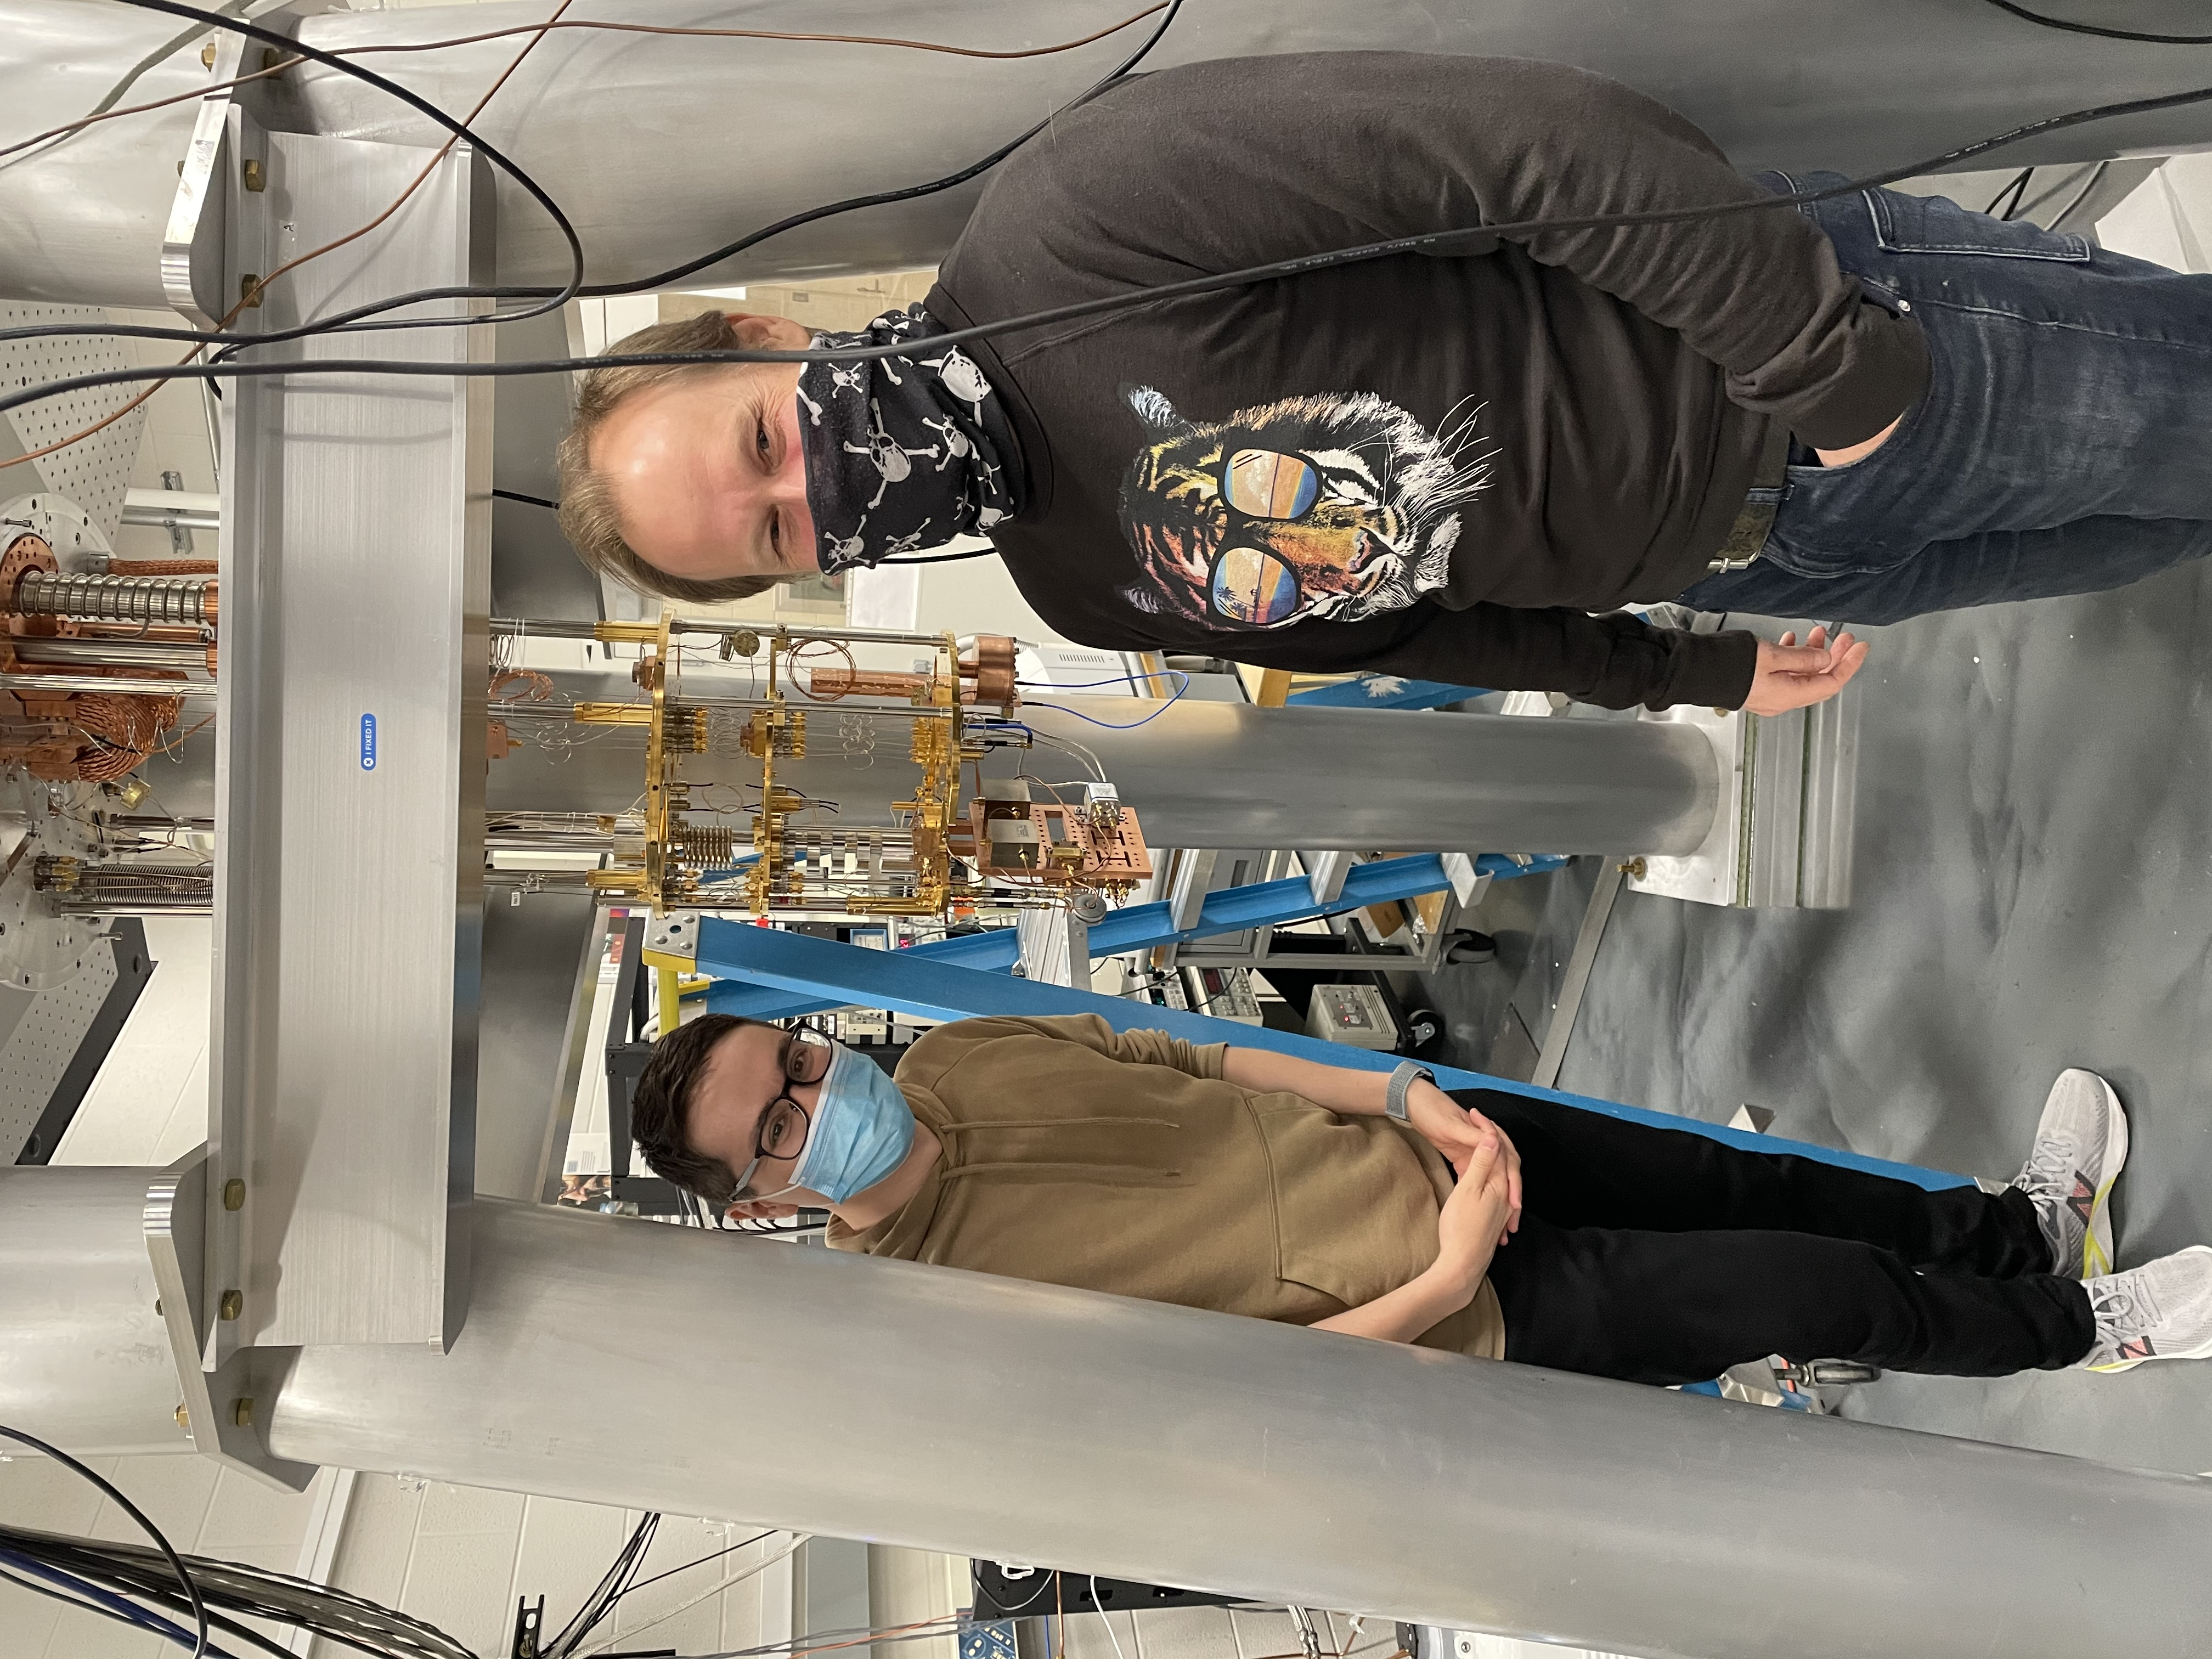
\includegraphics[width=1.3\textwidth]{qcfigures/lab.jpeg}}
      \end{center}
\end{columns}
      \end{footnotesize}
    }
\end{frame}

\begin{frame}
      \frametitle{Single electrons can make great qubits}
  {
      \begin{footnotesize}
     \begin{columns}
       \column{5.0cm}
\begin{alertblock}{Electrons on helium}
       At the heart is the trapping and control
       of individual electrons floating above pools of superfluid
       helium. These electrons form the qubits of apotential paltform  for quantum
       computer, and the purity of the superfluid helium protects the
       intrinsic quantum properties of each electron. The  ultimate
       goal is to build a large-scale quantum computer based on
       quantum magnetic (spin) state of these trapped electrons.
\end{alertblock}       
\column{5cm}
      \begin{center}
	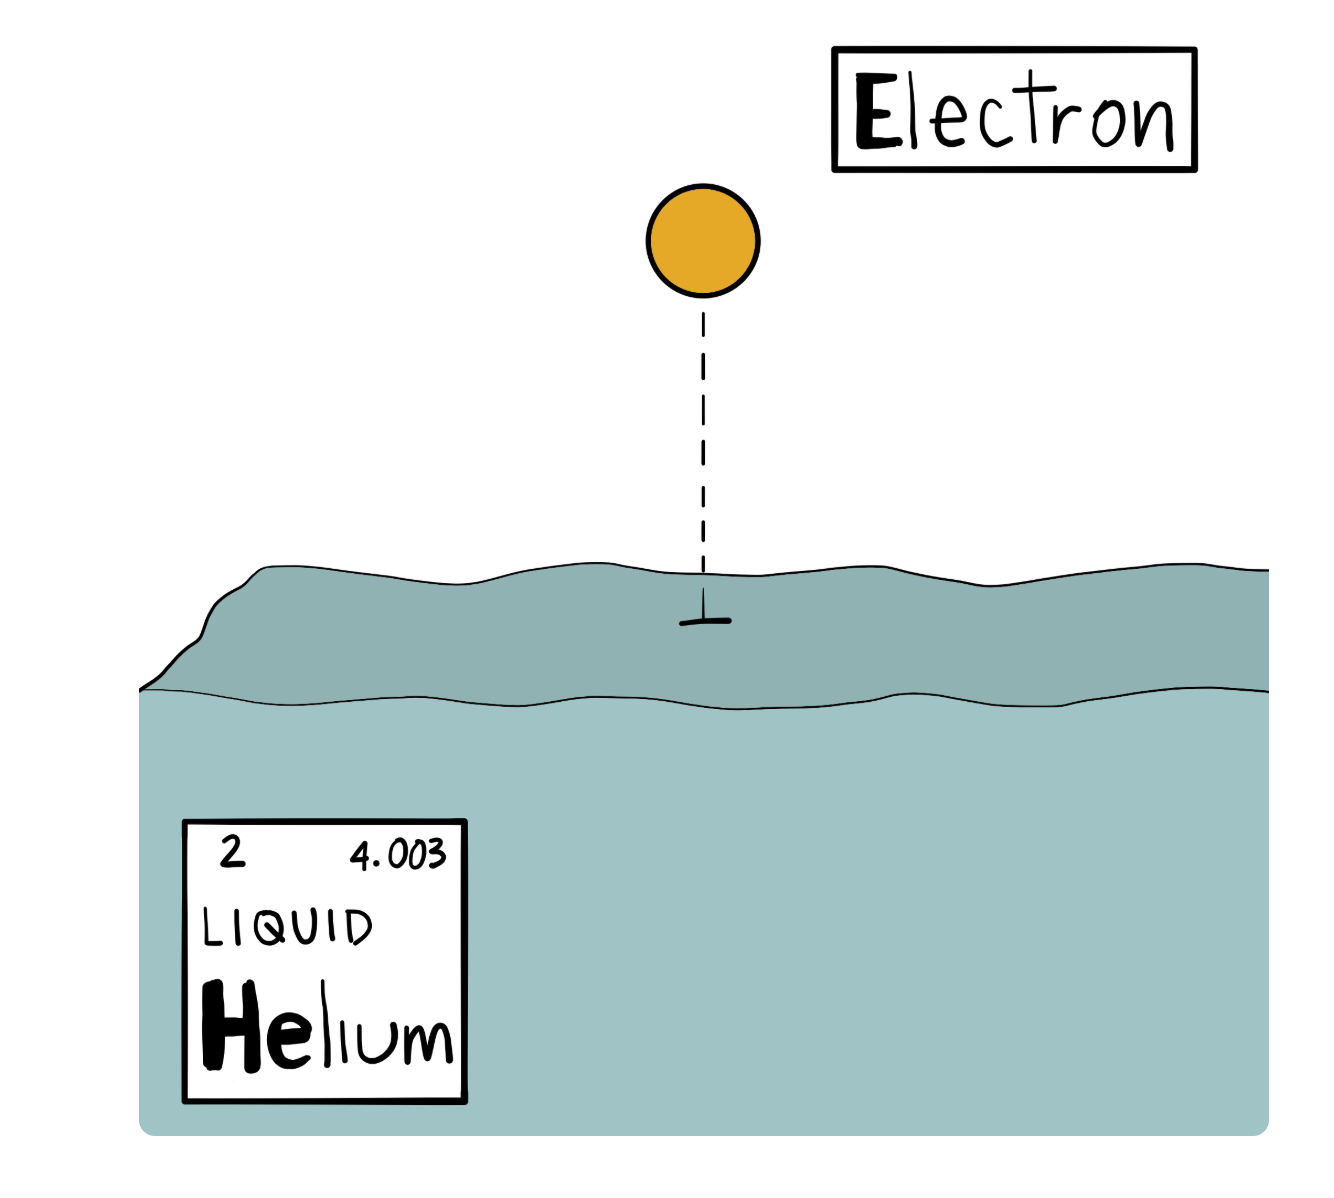
\includegraphics[width=1.2\textwidth]{qcfigures/nordicquantumfig1.png}
      \end{center}
\end{columns}
      \end{footnotesize}
    }
\end{frame}





\begin{frame}
      \frametitle{Operations for quantum computing}
  {

	
      \begin{footnotesize}
     \begin{columns}
       \column{5.0cm}
\begin{alertblock}{Electrons on helium}       
  Quantum information can be encoded in a number of ways using single electrons. Currently, we are working with the side-to-side(lateral) quantum motion of the electron in the engineered trap. This motion can either be in its lowest energy state, the ground state, or in a number of higher-energy excited states. This electron motion also provides the readout capabilities for the ultimate goal of building a large-scale quantum computer based on the electron's magnetic moment (spin).
  \end{alertblock}       
\column{5cm}
      \begin{center}
	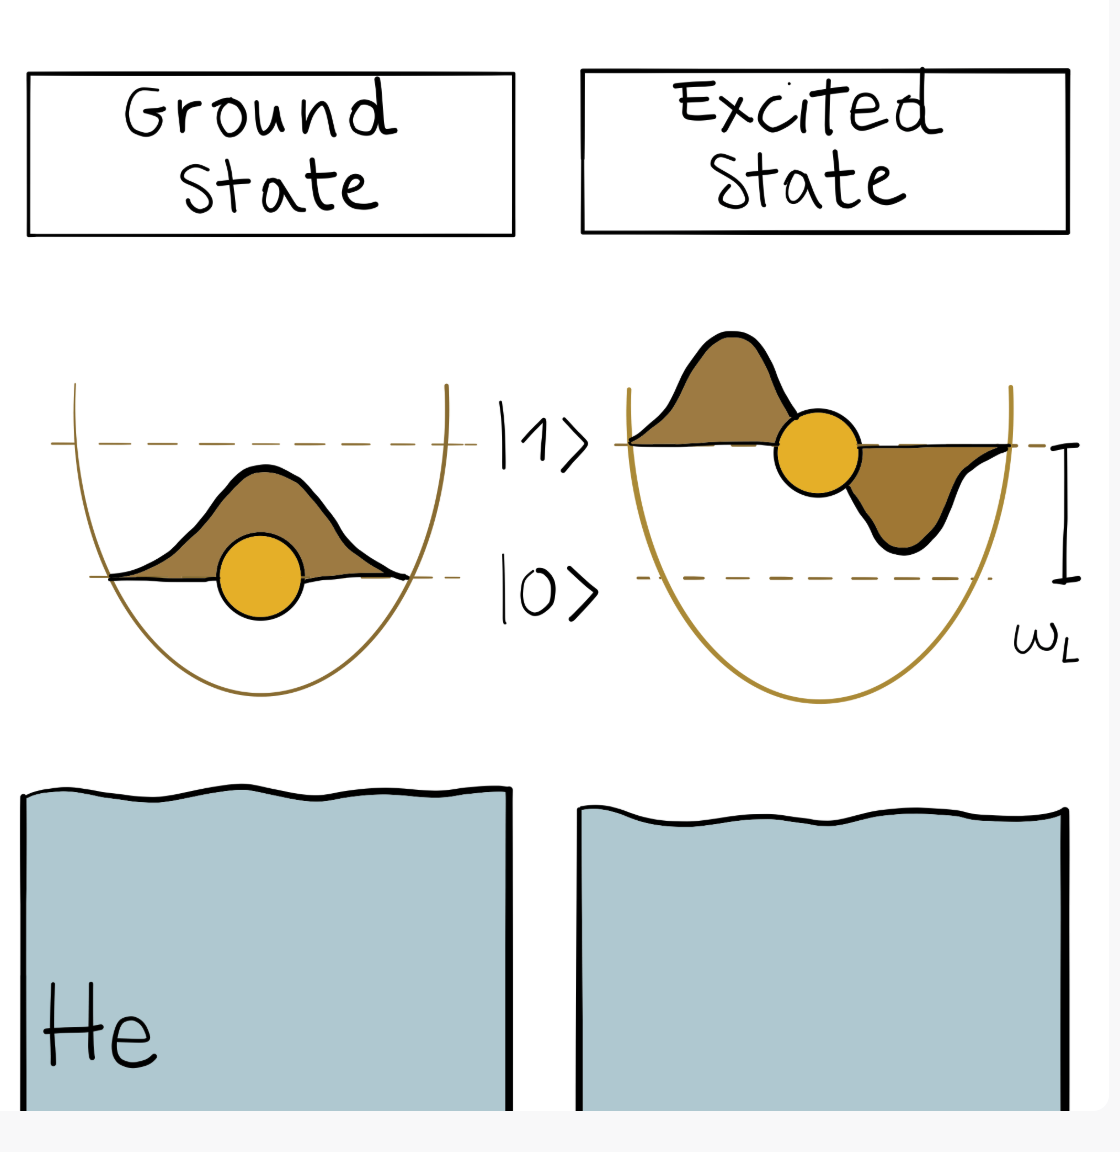
\includegraphics[width=1.2\textwidth]{qcfigures/nordicquantumfig4.png}
      \end{center}
\end{columns}
      \end{footnotesize}
    }
\end{frame}    



\begin{frame}
      \frametitle{Final experimental and theoretical  setup for Coulomb entanglement}
  {

	
      \begin{footnotesize}
     \begin{columns}
       \column{5.0cm}
\begin{enumerate}
\item Microdevice where two electrons are trapped in a double-well potential created by electrodes 1-7. The read-out is provided by two superconducting resonators dispersively coupled to  electron's in-plane motional states.

\item Coupling constants from each individual electrode beneath the helium layer.

\item The electron's energy in a  double-well electrostatic potential.
\item Screened Coulomb interaction
\end{enumerate}

\column{6cm}
      \begin{center}
	
\includegraphics[width=1.15\textwidth]{qcfigures/figure1.pdf}
      \end{center}
\end{columns}
      \end{footnotesize}
    }
\end{frame}

\begin{frame}[plain,fragile]
\frametitle{Recent work}

\begin{block}{}
\begin{itemize}
\item {\bf Coulomb interaction-driven entanglement of electrons on helium}, Niyaz R. Beysengulov {\em et al.}, PRX Quantum {\bf 5}, 030324 (2024).
\item {\bf Design and Dynamics of High-Fidelity Two-Qubit Gates with Electrons on Helium}, Oskar Leinonen {\em et al.}, Physical Review A {\bf 113}, 032624 (2026)
\item {\bf Electrons on Helium and Entangled Quantum Sensors for Particle Physics}, Niyaz R. Beysengulov {\em et al.}, Communications Physics, in preparation
\end{itemize}
\end{block}

\end{frame}



\begin{frame}{Two-Electron 2D Schrödinger via FCI with Slater Determinants}

\textbf{Key approach for identical fermions:}
\begin{itemize}
\item We construct the two-electron basis using \textbf{Slater determinants} that include both spatial and spin degrees of freedom
\item Each basis state is a properly antisymmetrized combination: $|\psi\rangle = |\phi_a \sigma_i; \phi_b \sigma_j\rangle$ where the total wavefunction is antisymmetric under particle exchange
\item This naturally separates states into singlet (spatially symmetric) and triplet (spatially antisymmetric) configurations
\item We include the full 2D soft Coulomb interaction and diagonalize the Hamiltonian in this antisymmetrized basis
\item We compute both spin expectation values ($\langle S^2 \rangle$, $\langle S_z \rangle$) and study the entanglement entropy for each eigenstate
\end{itemize}

\end{frame}

\begin{frame}{Double-Well Trap Potential}

We use an arbitrary 2D potential $V(x,y)$ for the single electrons, meant to represent the electrostatic trapping potential from electrodes beneath the helium surface. For simplicity here we show  an analytic double-well form:

\begin{itemize}
\item Quartic double well in x: $V_x = k(x^2 - a^2)^2$
\item Harmonic confinement in y: $V_y = \frac{1}{2}k_y y^2$
\end{itemize}
To allow specification of a 2D electrode geometry and voltages, one would solve the 3D Laplace equation for the electrode layout to find the coupling functions $\kappa_i(x,y)$ on the helium surface. Then the total trap potential is

$$V(x,y) = \sum_i \kappa_i(x,y)\,V_i$$


\end{frame}

\begin{frame}[plain,fragile]
\frametitle{Harmonic oscillator double well, no anharmonic terms}

%\vspace{6mm}

\centerline{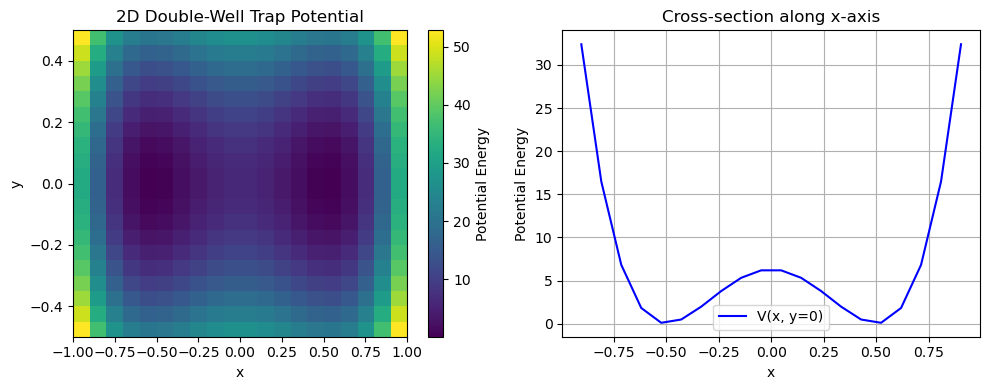
\includegraphics[width=0.9\linewidth]{qcfigures/figure_001.png}}

%\vspace{6mm}
\end{frame}



\begin{frame}{Two-Electron Slater Determinant Basis for Identical Fermions}

For \textbf{indistinguishable fermions}, we must construct properly antisymmetrized two-electron states using Slater determinants. Each basis state includes both spatial orbitals $\phi_i(\mathbf{r})$ and spin states $\sigma \in \{\uparrow, \downarrow\}$.

A two-electron Slater determinant is:
$$|\phi_a\sigma_i, \phi_b\sigma_j\rangle = \frac{1}{\sqrt{2}}\begin{vmatrix} \phi_a(\mathbf{r}_1)\sigma_i(1) & \phi_b(\mathbf{r}_1)\sigma_j(1) \\ \phi_a(\mathbf{r}_2)\sigma_i(2) & \phi_b(\mathbf{r}_2)\sigma_j(2) \end{vmatrix}$$

For each eigenstate in our Slater determinant basis, we compute:
1. \textbf{Spin expectation values}: $\langle S^2 \rangle$ and $\langle S_z \rangle$
2. \textbf{Total entanglement entropy}: Via Schmidt decomposition including both spin and spatial degrees of freedom

\end{frame}

\begin{frame}{Why compute total (spatial + spin) entanglement?}

For \textbf{indistinguishable fermions}, the spatial and spin degrees of freedom are fundamentally coupled by antisymmetrization:
\begin{itemize}
\item \textbf{Singlet states}: Spatially symmetric × spin antisymmetric
\item \textbf{Triplet states}: Spatially antisymmetric × spin symmetric
\end{itemize}
This coupling means that \textbf{pure spatial entanglement alone would often be zero} because:
\begin{itemize}
\item For a pure singlet in orbital |a,a⟩, there's only one spatial configuration (both electrons in the same orbital)
\item The entanglement comes from the spin antisymmetry: $(|\uparrow\downarrow\rangle - |\downarrow\uparrow\rangle)/\sqrt{2}$
\end{itemize}
The \textbf{total entanglement} (including both spin and spatial) captures the full quantum correlations between the two particles and is the physically meaningful measure for identical fermions.  We use {\em Model-aware Reinforcement Learning} to optimize the various parameters in order to maximize entanglement.

\end{frame}


\begin{frame}{What is Reinforcement Learning? (Used here to maximize entanglement)}
\begin{block}{Setting: electrons on helium}
In our double-well setup, the \textbf{agent} controls the electrode voltages $\{V_i\}$; the \textbf{reward} is the total entanglement entropy of the two-electron state. RL finds the voltage configuration that maximizes quantum correlations.
\end{block}

\begin{block}{General framework}  

The RL framework consists of an {\bf agent} that learns how to solve a
task by interacting with a physical system, called the
environment. The agent can select {\bf actions} that modify the {\bf
  state} of the environment; as a consequence a {\bf reward} is given
to the agent, and the process repeats in a positive feedback loop. The
objective is to maximize the sum of expected rewards and thereby
accomplish the task. The agent learns a {\bf strategy} that can be
employed under similar yet different circumstances. The so-called {\bf
  policy} is the rule for choosing actions.

\end{block}
\end{frame}


\begin{frame}{Machine learning meets quantum hardware}

  \begin{columns}[T]
    \begin{column}{0.52\textwidth}
      \textbf{Core challenge:} Quantum devices are delicate systems.
      Small imperfections $\Rightarrow$ decoherence and loss of information.

      \bigskip
      \textbf{Reinforcement learning} has proven particularly powerful:
      \begin{itemize}
        \item Agent interacts with a simulated/experimental quantum system
        \item Learns control protocols that optimize a desired objective
        \item Applications: state preparation, high-fidelity gate implementation
      \end{itemize}
    \end{column}
    \begin{column}{0.44\textwidth}
      \begin{block}{ML Applications to Quantum Hardware}
        \begin{itemize}
          \item Calibration \& characterisation
          \item Error mitigation \& noise reduction
          \item Automated control-sequence discovery
          \item Adaptive quantum experiment design
        \end{itemize}
      \end{block}
      \medskip
      \small Parameter spaces in quantum devices are \textbf{huge}
      — traditional optimization struggles.
    \end{column}
  \end{columns}

\end{frame}


\begin{frame}{Conceptual Framework — Three Pillars of Future Discovery}
\centerline{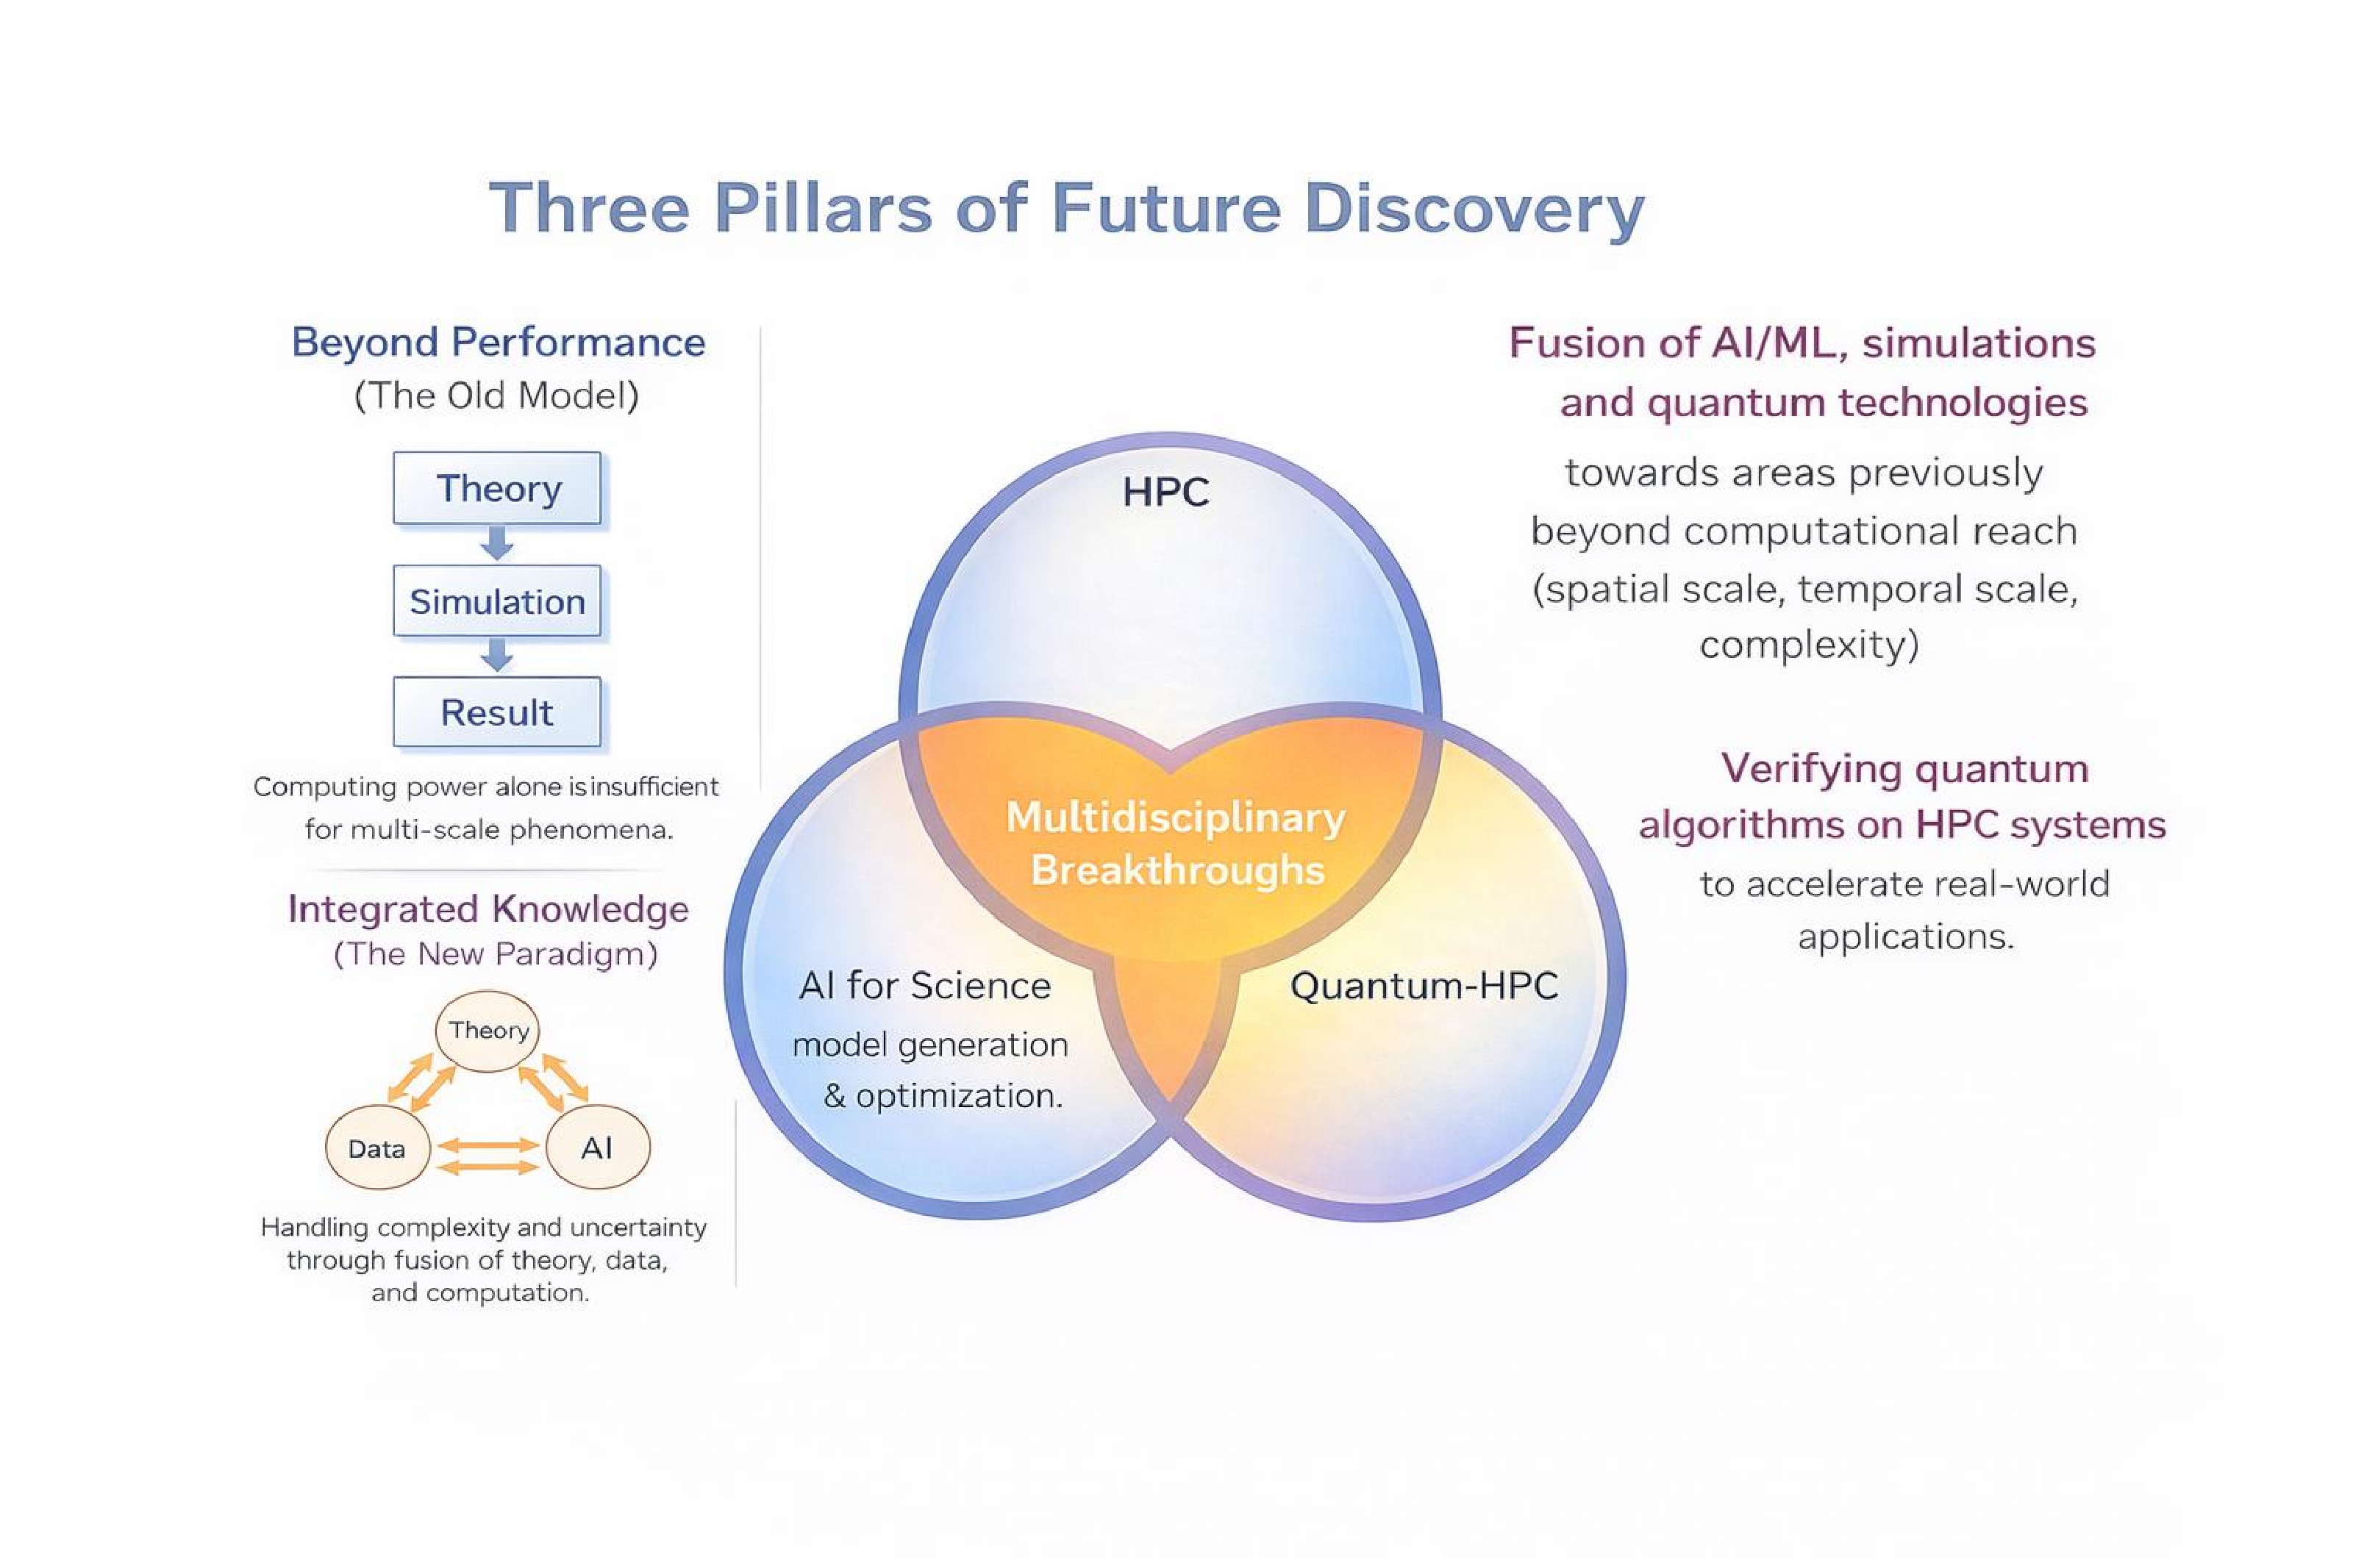
\includegraphics[width=0.85\linewidth]{Futurevision.pdf}}

\end{frame}




\begin{frame}{Quantum Control}
\centerline{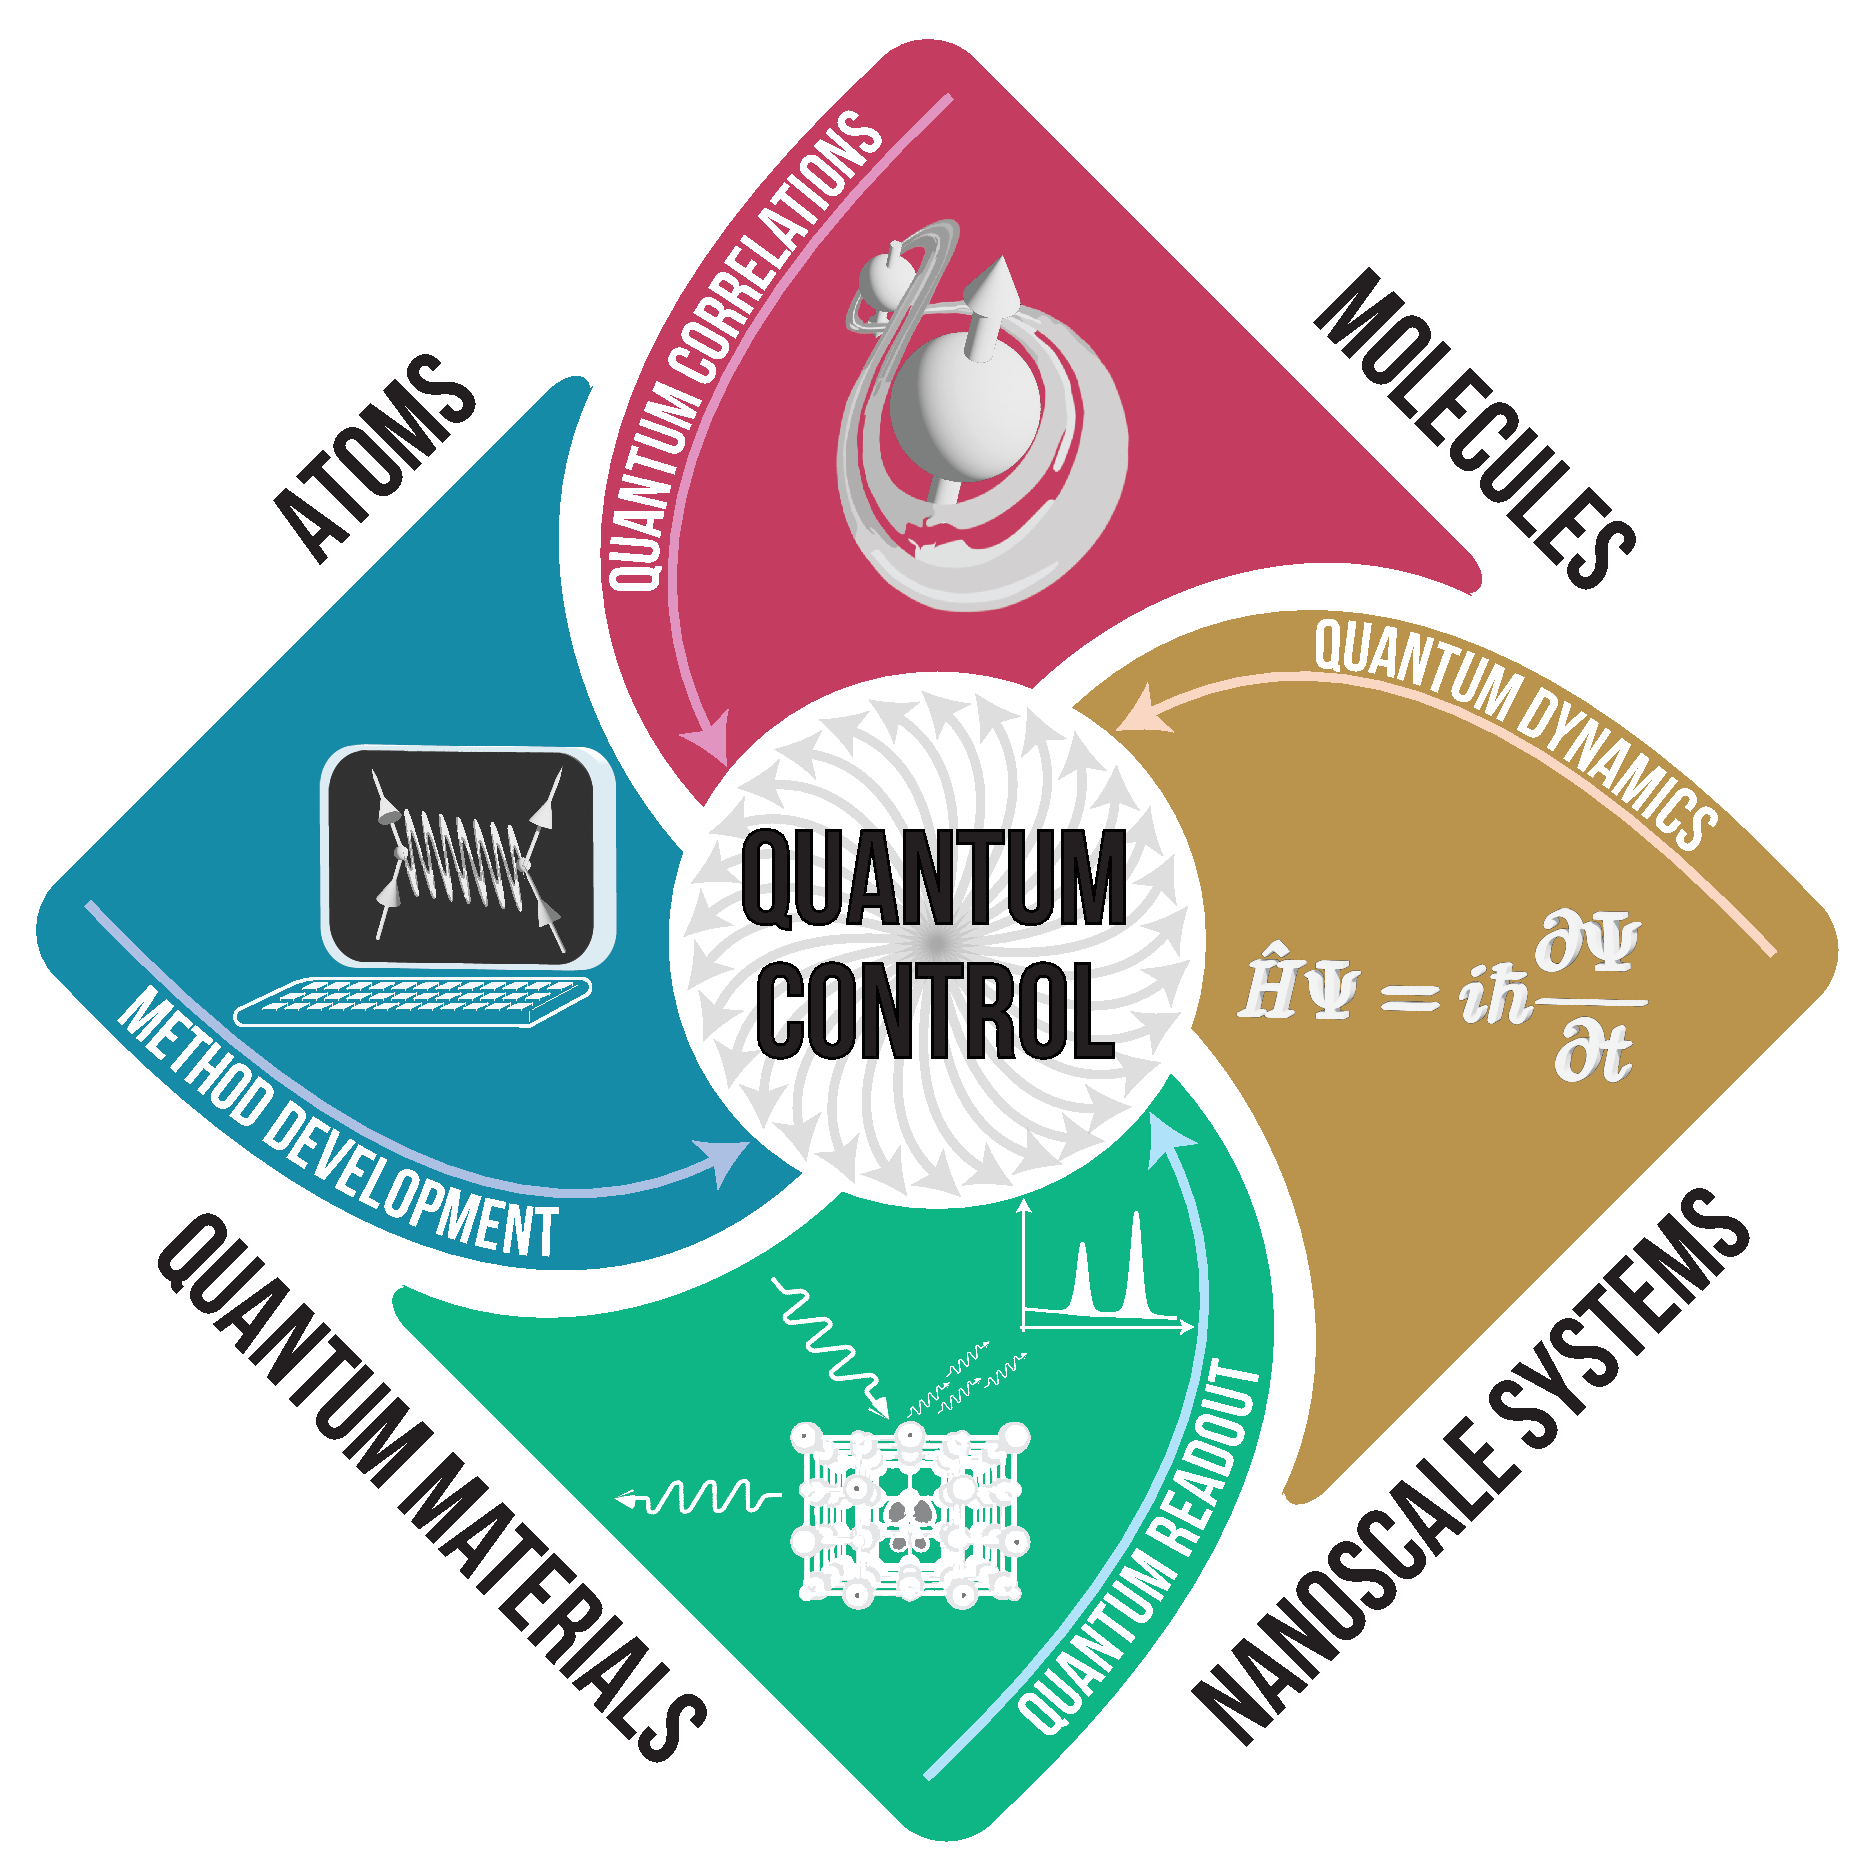
\includegraphics[width=0.5\linewidth]{quantumcontrol.pdf}}
\end{frame}



\begin{frame}{Neural Paradigms for Quantum Many-Body Problems}
  \renewcommand{\arraystretch}{1.35}
  \begin{tabular}{p{2.6cm}p{4.0cm}p{4.6cm}}
    \toprule
    \textbf{Method} & \textbf{Core idea} & \textbf{Natural regime} \\
    \midrule
    Variational MC (VMC) with neural ansatz &
      Minimise $\langle H\rangle$ via MC sampling &
      Large $N$, ground states, lattice systems \\
    \alert{PINNs} &
      Enforce PDE and symmetry residuals directly in loss &
      Continuous space, complex geometries, dynamics \\
    \bottomrule
  \end{tabular}

  \vspace{0.5cm}
  \begin{alertblock}{Key PINN advantage for quantum dots}
    Wave function learned as a continuous function
    of particle coordinates; antisymmetry, normalization, and conservation
    laws imposed as explicit constraints or penalty terms.
  \end{alertblock}
\end{frame}

%% ============================================================
\section{Physics-Informed Neural Networks}
%% ============================================================

%%
\begin{frame}{PINN Formulation}
  Let $u:\Omega\subset\mathbb{R}^d\to\mathbb{R}$ satisfy
  $\mathcal{N}[u](x)=0$ on $\Omega$ with $u=g$ on $\partial\Omega$.
  \medskip

  A PINN represents $u$ by a neural network $u_\theta(x)$ and minimises:
  \begin{equation*}
    \mathcal{L}(\theta)
    = \lambda_{\rm data}\!\sum_i|u_\theta(x_i)-y_i|^2
    + \lambda_{\rm PDE}\!\sum_j|\mathcal{N}[u_\theta](\xi_j)|^2
    + \lambda_{\rm BC}\!\sum_k|u_\theta(\zeta_k)-g(\zeta_k)|^2
  \end{equation*}

  \begin{columns}[T]
    \column{0.32\textwidth}
      \begin{block}{Data term}
        Observed data $\{x_i,y_i\}$
      \end{block}
    \column{0.32\textwidth}
      \begin{block}{PDE residual}
        Collocation points $\xi_j$ in $\Omega$
      \end{block}
    \column{0.32\textwidth}
      \begin{block}{BC term}
        Boundary pts $\zeta_k$ on $\partial\Omega$
      \end{block}
  \end{columns}

  \vspace{0.4cm}
  \textbf{Key tool — Automatic differentiation (AD):} evaluates
  $\nabla u_\theta$ and $\Delta u_\theta$ exactly (to floating-point
  precision), enabling end-to-end training constrained by physical laws.
\end{frame}

%%


%%
\begin{frame}{Mitigation Strategies and Biases}
  Generalization in physics ML means \alert{consistency with physical laws},
  not merely accuracy on unseen data. Three interacting mechanisms:
  \begin{enumerate}
    \item Algorithmic stability of gradient-based optimization
    \item Implicit bias toward smooth, low-complexity solutions
    \item Architectural inductive biases encoding domain knowledge
  \end{enumerate}

  \vspace{0.3cm}
  \begin{block}{Practical engineering checklist}
    \small
    \begin{columns}[T]
      \column{0.48\textwidth}
        \begin{itemize}
          \item Weak/variational or energy formulations when strong form
                is unstable
          \item Hard-enforce essential boundary conditions
          \item Balance various loss terms
        \end{itemize}
      \column{0.48\textwidth}
        \begin{itemize}
          \item Smooth activations; architectures controlling derivatives
          \item Exploit symmetry and equivariance
          \item Second-order optimizers (L-BFGS, Stochastic Reconfiguration)
          \item Importance/stratified sampling; space-time protocols
        \end{itemize}
    \end{columns}
  \end{block}
\end{frame}

%% ─── Variational limits: does a PINN respect the variational principle? ─────
\begin{frame}{Does a PINN Respect the Variational Principle?}
  \begin{itemize}
    \item Physics-Informed Neural Networks (PINNs) are increasingly used
          to solve quantum many-body problems.
    \item A central question:
  \end{itemize}

  \vspace{0.2cm}
  \begin{block}{Key question}
    Does a PINN approximation to the ground-state energy respect the
    variational principle?
  \end{block}

  \vspace{0.2cm}
  \begin{itemize}
    \item The answer depends crucially on how the PINN loss is formulated.
    \item Two strategies — \alert{variational} and \alert{residual-based} —
          have fundamentally different properties.
  \end{itemize}
\end{frame}

\begin{frame}{The Variational Principle}
  For a normalized trial wave function $\psi_\theta$:
  \[
    E[\psi_\theta]
    = \frac{\langle\psi_\theta|H|\psi_\theta\rangle}
           {\langle\psi_\theta|\psi_\theta\rangle}
    \geq E_0
  \]

  \begin{columns}[T]
    \column{0.48\textwidth}
      \begin{itemize}
        \item $E_0$: exact ground-state energy
        \item Equality holds \emph{only} for the exact ground state
      \end{itemize}
    \column{0.48\textwidth}
      \begin{block}{Key property}
        Any admissible trial state gives an \textbf{upper bound} to the
        true ground-state energy.
      \end{block}
  \end{columns}
\end{frame}

\begin{frame}{Two PINN Training Strategies}
  A PINN represents the wave function as a neural network.
  \vspace{0.3cm}
  \begin{columns}[T]
    \column{0.48\textwidth}
      \begin{block}{1.\ Variational (energy-based)}
        \[
          \mathcal{L}(\theta)
          = \frac{\langle\psi_\theta|H|\psi_\theta\rangle}
                 {\langle\psi_\theta|\psi_\theta\rangle}
        \]
        Equivalent to Rayleigh--Ritz minimisation.\\
        \alert{Variational principle preserved:}
        $E_\theta \geq E_0$.
      \end{block}
    \column{0.48\textwidth}
      \begin{alertblock}{2.\ Residual minimisation (PDE-based)}
        \[
          \mathcal{L}(\theta)
          = \bigl\|(H-E)\psi_\theta\bigr\|^2
        \]
        Enforces the Schr\"{o}dinger equation directly.\\
        Residual minimisation $\neq$ energy minimisation.
      \end{alertblock}
  \end{columns}
\end{frame}

\begin{frame}{Breakdown of the Variational Property}
  \begin{columns}[T]
    \column{0.52\textwidth}
      For residual-based PINNs there is \textbf{no guarantee} that:
      \[
        E_\theta \geq E_0
      \]
      Possible failure modes:
      \begin{itemize}
        \item Energies \emph{below} the true ground state
        \item Convergence to incorrect eigenstates
        \item Residual small but solution error large
              (stability issues)
      \end{itemize}
    \column{0.44\textwidth}
      \begin{alertblock}{Conclusion}
        Residual-based PINNs do \textbf{not} preserve the variational
        principle.
      \end{alertblock}
      \vspace{0.3cm}
      \begin{block}{Connection to PINN challenges}
        This is a manifestation of the \emph{stability} challenge:
        small PDE residual $\not\Rightarrow$ small energy error.
      \end{block}
  \end{columns}
\end{frame}

\begin{frame}{Key Practical Issues}
  \begin{columns}[T]
    \column{0.48\textwidth}
      \textbf{Normalization}
      \begin{itemize}
        \item Must be enforced explicitly or via the energy quotient
        \item Unnormalized networks can give arbitrarily low apparent energies
      \end{itemize}
      \vspace{0.3cm}
      \textbf{Symmetry constraints}
      \begin{itemize}
        \item Fermionic antisymmetry (Slater determinant)
        \item Spin and spatial symmetries
      \end{itemize}
    \column{0.48\textwidth}
      \textbf{Nodal structure}
      \begin{itemize}
        \item Especially critical for fermions
        \item Incorrect nodes $\Rightarrow$ incorrect ground state
      \end{itemize}
      \vspace{0.3cm}
      \textbf{Boundary conditions}
      \begin{itemize}
        \item Hard enforcement preferred over soft penalties
        \item Soft boundary conditions can be dominated by other loss terms
      \end{itemize}
  \end{columns}
\end{frame}

\begin{frame}{Hybrid Loss Functions}
  A common approach combining the best of both strategies:
  \[
    \mathcal{L}(\theta)
    = \frac{\langle\psi_\theta|H|\psi_\theta\rangle}
           {\langle\psi_\theta|\psi_\theta\rangle}
    + \lambda\,\mathcal{L}_{\text{BC}}
    + \mu\,\mathcal{L}_{\text{sym}}
  \]

  \begin{columns}[T]
    \column{0.52\textwidth}
      \begin{itemize}
        \item Energy (Rayleigh--Ritz) term preserves variational character
        \item $\mathcal{L}_{\text{BC}}$: boundary-condition penalty
        \item $\mathcal{L}_{\text{sym}}$: symmetry (antisymmetry, spin) penalty
      \end{itemize}
    \column{0.44\textwidth}
      \begin{block}{Recommendation}
        Avoid making the PDE residual the \emph{dominant} loss term
        if variational upper bounds are required.
        Use the energy quotient as the primary objective.
      \end{block}
  \end{columns}
\end{frame}

\begin{frame}{Variational vs.\ Residual: Summary Comparison}
  \renewcommand{\arraystretch}{1.35}
  \begin{tabular}{p{3.2cm} p{4.0cm} p{4.0cm}}
    \toprule
    \textbf{Property} & \textbf{Variational PINN} & \textbf{Residual PINN} \\
    \midrule
    Loss function      & $\langle\psi_\theta|H|\psi_\theta\rangle/\|\psi_\theta\|^2$
                       & $\|(H-E)\psi_\theta\|^2$ \\
    Variational bound  & \alert{Yes}: $E_\theta\geq E_0$ & No guarantee \\
    Enforces PDE       & Implicitly (at minimum)   & Explicitly \\
    Normalization      & Automatic via quotient    & Must be added \\
    Risk of sub-$E_0$  & None                      & Present \\
    Connection to QMC  & Direct (Rayleigh--Ritz)   & Indirect \\
    \bottomrule
  \end{tabular}
\end{frame}

\begin{frame}{Variational Structure: Takeaways}
  \begin{columns}[T]
    \column{0.52\textwidth}
      \begin{block}{When variational principle is preserved}
        \begin{itemize}
          \item Loss $\equiv$ energy Rayleigh quotient
          \item Normalization enforced via quotient
          \item Antisymmetry exact (Slater determinant)
          \item SR / natural-gradient optimization tail
        \end{itemize}
      \end{block}
    \column{0.44\textwidth}
      \begin{alertblock}{When it is not}
        \begin{itemize}
          \item Dominant PDE residual loss
          \item Soft normalization penalty
          \item No antisymmetry architecture
          \item Pure gradient-descent on residual
        \end{itemize}
      \end{alertblock}
  \end{columns}

  \vspace{0.4cm}
  \begin{center}
    \large
    \textbf{Variational structure must be built into the loss function.}
  \end{center}
\end{frame}

%% ============================================================
\section{The Ansatz}
%% ============================================================

%%
\begin{frame}{Ansatz: Slater--Jastrow--Neural Correlator}
  \begin{equation*}
    \Psi_{\theta,\beta}(R)
    = \underbrace{\mathrm{SD}(R')}_{\text{antisymmetry}}\;
      \exp\!\bigl(
        \underbrace{U(R)}_{\text{analytic pair}}
        +\underbrace{W_\theta(R)}_{\text{neural correlator}}
      \bigr),
    \qquad
    R' = R + \underbrace{\Delta_\beta(R)}_{\text{backflow}}
  \end{equation*}

  \vspace{0.2cm}
  \begin{columns}[T]
    \column{0.52\textwidth}
      \begin{block}{Four components}
        \begin{itemize}
          \item $\mathrm{SD}(R')$ — Slater determinant: exact fermionic
                antisymmetry
          \item $U(R)$ — analytic cusp/pair term (evaluated on \emph{unscaled}
                distances $r_{ij}$)
          \item $W_\theta(R)$ — compact permutation-invariant neural correlator
                (evaluated on \emph{trap-scaled} coords $\tilde{\mathbf x}_i
                = \sqrt\omega\,\mathbf x_i$)
          \item $\Delta_\beta(R)$ — optional backflow, only inside $\mathrm{SD}$
        \end{itemize}
      \end{block}
    \column{0.44\textwidth}
      \begin{alertblock}{Coordinate convention}
        $W_\theta$ uses trap-scaled $\tilde{\mathbf x}_i=\sqrt\omega\,\mathbf x_i$;
        $U$ uses physical $r_{ij}$.\\[5pt]
        This separates the length scales set by the trap from those set by the
        Coulomb interaction.
      \end{alertblock}
      \vspace{0.3cm}
      Two backflow variants:\\
      \textbf{PINN+BF} (\texttt{BackflowNet}) and\\
      \textbf{PINN+CTNN} (\texttt{CTNNBackflowNet})
  \end{columns}
\end{frame}

%%
\begin{frame}{Analytic Pair Term and Backflow Modules}
  \begin{columns}[T]
    \column{0.48\textwidth}
      \begin{block}{Analytic cusp pair term $U(R)$}
        \[
          U(R)=\sum_{i<j} u_{\sigma_i\sigma_j}(r_{ij}),\quad
          u_{\sigma\sigma'}(r)=\gamma_{\sigma\sigma'}\,r\,e^{-r}
        \]
        Spin-dependent couplings satisfying cusp conditions:
        \[
          \gamma_{\uparrow\downarrow}=\tfrac{1}{d-1},\qquad
          \gamma_{\uparrow\uparrow}=\tfrac{1}{d+1}
        \]
        Evaluated on \emph{unscaled} distances $r_{ij}=\|\mathbf x_i-\mathbf x_j\|$.
      \end{block}
    \column{0.48\textwidth}
      \begin{block}{Backflow $\Delta_\beta(R)$}
        Shifts only the Slater determinant: $R'=R+\Delta_\beta(R)$.

        \smallskip
        \textbf{\texttt{BackflowNet}}: pairwise message-passing MLP;
        output $s_\beta\tanh(\delta\mathbf x_i)$.

        \smallskip
        \textbf{\texttt{CTNNBackflowNet}}: explicit node features $\mathbf h_i\in\mathbb R^{H_v}$ and
        edge features $\mathbf h_{ij}\in\mathbb R^{H_e}$; learned
        linear transports between node and edge spaces.
      \end{block}
  \end{columns}
\end{frame}



%% ============================================================
\section{Results: Ground-State Energies}
%% ============================================================



%% ─── Results begin here ─────────────────────────────────────────────────────

%%
\begin{frame}{Ground-State Energies: Comparison with DMC}
  \scriptsize
  \renewcommand{\arraystretch}{1.20}
  \begin{tabular}{c|c|c|cc|cc}
    \toprule
    $N$ & $\omega$ & DMC reference & PINN+BF & \%\,err & PINN+CTNN & \%\,err \\
    \midrule
    2 & 0.01  & $0.073839(2)$  & $0.073838(1)$ & $-0.0014$ & $0.0738382(5)$ & $-0.0014$ \\
      & 1.00  & $3.00000$      & $2.99999(1)$  & $-0.0003$ & $3.00000(2)$   & $-0.0000$ \\
    \midrule
    6 & 0.10  & $3.55385(5)$   & $3.5549(1)$   & $+0.030$  & $\mathbf{3.55388(5)}$ & $+0.0008$ \\
      & 0.50  & $11.78484(6)$  & $11.7895(4)$  & $+0.040$  & $\mathbf{11.7847(2)}$ & $-0.0000$ \\
      & 1.00  & $20.15932(8)$  & $20.1610(6)$  & $+0.008$  & $\mathbf{20.1585(3)}$ & $-0.004$  \\
    \midrule
    12& 0.50  & $39.1596(1)$   & $39.1786(8)$  & $+0.049$  & $\mathbf{39.1604(3)}$ & $+0.002$  \\
      & 1.00  & $65.7001(1)$   & $65.717(1)$   & $+0.026$  & $\mathbf{65.69556(5)}$& $-0.007$  \\
    \midrule
    20& 0.10  & $29.9779(1)$   & ---           & ---       & $29.9888(2)$          & $+0.036$  \\
      & 0.50  & $93.8752(1)$   & ---           & ---       & $\mathbf{93.8789(5)}$ & $+0.004$  \\
      & 1.00  & $155.8822(1)$  & ---           & ---       & $\mathbf{155.8738(7)}$& $-0.002$  \\
    \bottomrule
  \end{tabular}
  \normalsize

  \vspace{0.25cm}
  \begin{itemize}
    \item $N=2$: both ans\"atze reproduce DMC within statistical error for
          all $\omega$
    \item $N\ge6$: PINN+CTNN systematically more accurate than PINN+BF
    \item $N=20$: CTNN remains accurate at scale; errors $\lesssim 0.04\%$
  \end{itemize}
\end{frame}


\begin{frame}[allowframebreaks]{Full Ground-State Energy Table}
  \scriptsize
  \renewcommand{\arraystretch}{1.15}
  \begin{tabular}{c|c|c|cc|cc}
    \toprule
    $N$ & $\omega$ & DMC ref. & PINN+BF & \%\,err & PINN+CTNN & \%\,err \\
    \midrule
    2 & $10^{-3}$ & ---            & $0.0137948(8)$ & ---        & $0.013778(1)$    & ---      \\
      & $10^{-2}$ & $0.073839(2)$  & $0.073838(1)$  & $-0.0014$ & $0.0738382(5)$   & $-0.0014$\\
      & $0.10$    & $0.44079(1)$   & $0.44079(1)$   & $+0.0000$ & $0.440796(4)$    & $-0.0000$\\
      & $0.50$    & $1.65977(1)$   & $1.65976(2)$   & $-0.0006$ & $1.65976(1)$     & $-0.0006$\\
      & $1.00$    & $3.00000$      & $2.99999(1)$   & $-0.0003$ & $3.00000(2)$     & $-0.0000$\\
    \midrule
    6 & $10^{-3}$ & ---            & $0.140913(1)$  & ---        & $0.1408172(7)$   & ---      \\
      & $10^{-2}$ & ---            & $0.69125(2)$   & ---        & $0.69036(1)$     & ---      \\
      & $0.10$    & $3.55385(5)$   & $3.5549(1)$    & $+0.0295$ & $3.55388(5)$     & $+0.0008$\\
      & $0.50$    & $11.78484(6)$  & $11.7895(4)$   & $+0.0395$ & $11.7847(2)$     & $-0.0000$\\
      & $1.00$    & $20.15932(8)$  & $20.1610(6)$   & $+0.0083$ & $20.1585(3)$     & $-0.0041$\\
    \midrule
    12& $10^{-3}$ & ---            & $0.515823(3)$  & ---        & $0.515365(4)$    & ---      \\
      & $10^{-2}$ & ---            & $2.48620(5)$   & ---        & $2.47363(4)$     & ---      \\
      & $0.10$    & $12.26984(8)$  & $12.2731(2)$   & $+0.0160$ & $12.2718(1)$     & ---      \\
      & $0.50$    & $39.1596(1)$   & $39.1786(8)$   & $+0.0485$ & $39.1604(3)$     & $+0.0018$\\
      & $1.00$    & $65.7001(1)$   & $65.717(1)$    & $+0.0257$ & $65.69556(5)$    & $-0.0069$\\
    \midrule
    20& $10^{-3}$ & ---            & ---            & ---        & $1.293033(6)$    & ---      \\
      & $10^{-2}$ & ---            & ---            & ---        & $6.14645(5)$     & ---      \\
      & $0.10$    & $29.9779(1)$   & ---            & ---        & $29.9888(2)$     & $+0.0364$\\
      & $0.50$    & $93.8752(1)$   & ---            & ---        & $93.8789(5)$     & $+0.0040$\\
      & $1.00$    & $155.8822(1)$  & ---            & ---        & $155.8738(7)$    & $-0.0024$\\
    \bottomrule
  \end{tabular}
\end{frame}



%%
\begin{frame}{Energy Partitioning: Approaching the Wigner Regime}
  \begin{columns}[T]
    \column{0.52\textwidth}
      Total energy decomposition:
      \[
        E = \langle T\rangle
            + \langle V_{\rm int}\rangle
            + \langle V_{\rm trap}\rangle
      \]
      Two diagnostics tracking interaction dominance:
      \[
        \Gamma(\omega)
        = \frac{\langle V_{\rm int}\rangle}{\langle T\rangle},\qquad
        \mathcal{C}(\omega)
        = \frac{2\langle V_{\rm trap}\rangle}{\langle V_{\rm int}\rangle}
      \]
      \begin{itemize}
        \item $\Gamma\!\uparrow$ as $\omega\!\downarrow$: interactions dominate
        \item $\mathcal{C}\to 1$: quasi-classical trap--Coulomb balance
      \end{itemize}
    \column{0.44\textwidth}
      \scriptsize
      \renewcommand{\arraystretch}{1.2}
      \begin{tabular}{c|cc|cc}
        \toprule
        $N$ & $\Gamma_{\omega=1}$ & $\mathcal{C}_{\omega=1}$
            & $\Gamma_{\omega=10^{-3}}$ & $\mathcal{C}_{\omega=10^{-3}}$ \\
        \midrule
        2  & 0.93 & 3.14 & 8.64  & 1.226 \\
        6  & 2.41 & 1.83 & 24.55 & 1.074 \\
        12 & 3.61 & 1.56 & 41.11 & 1.049 \\
        20 & 4.66 & 1.43 & 57.26 & 1.038 \\
        \bottomrule
      \end{tabular}
      \normalsize
      \vspace{0.3cm}
      \begin{alertblock}{Key trend}
        At $\omega=10^{-3}$, $N\ge 12$: $\mathcal{C}< 1.05$, i.e.\
        $V_{\rm int}\approx 2V_{\rm trap}$ to $\lesssim 5\%$.
      \end{alertblock}
  \end{columns}
\end{frame}

%%
\begin{frame}{Energy-Partition Diagnostics}
  \begin{columns}[T]
    \column{0.49\textwidth}
      \centering
      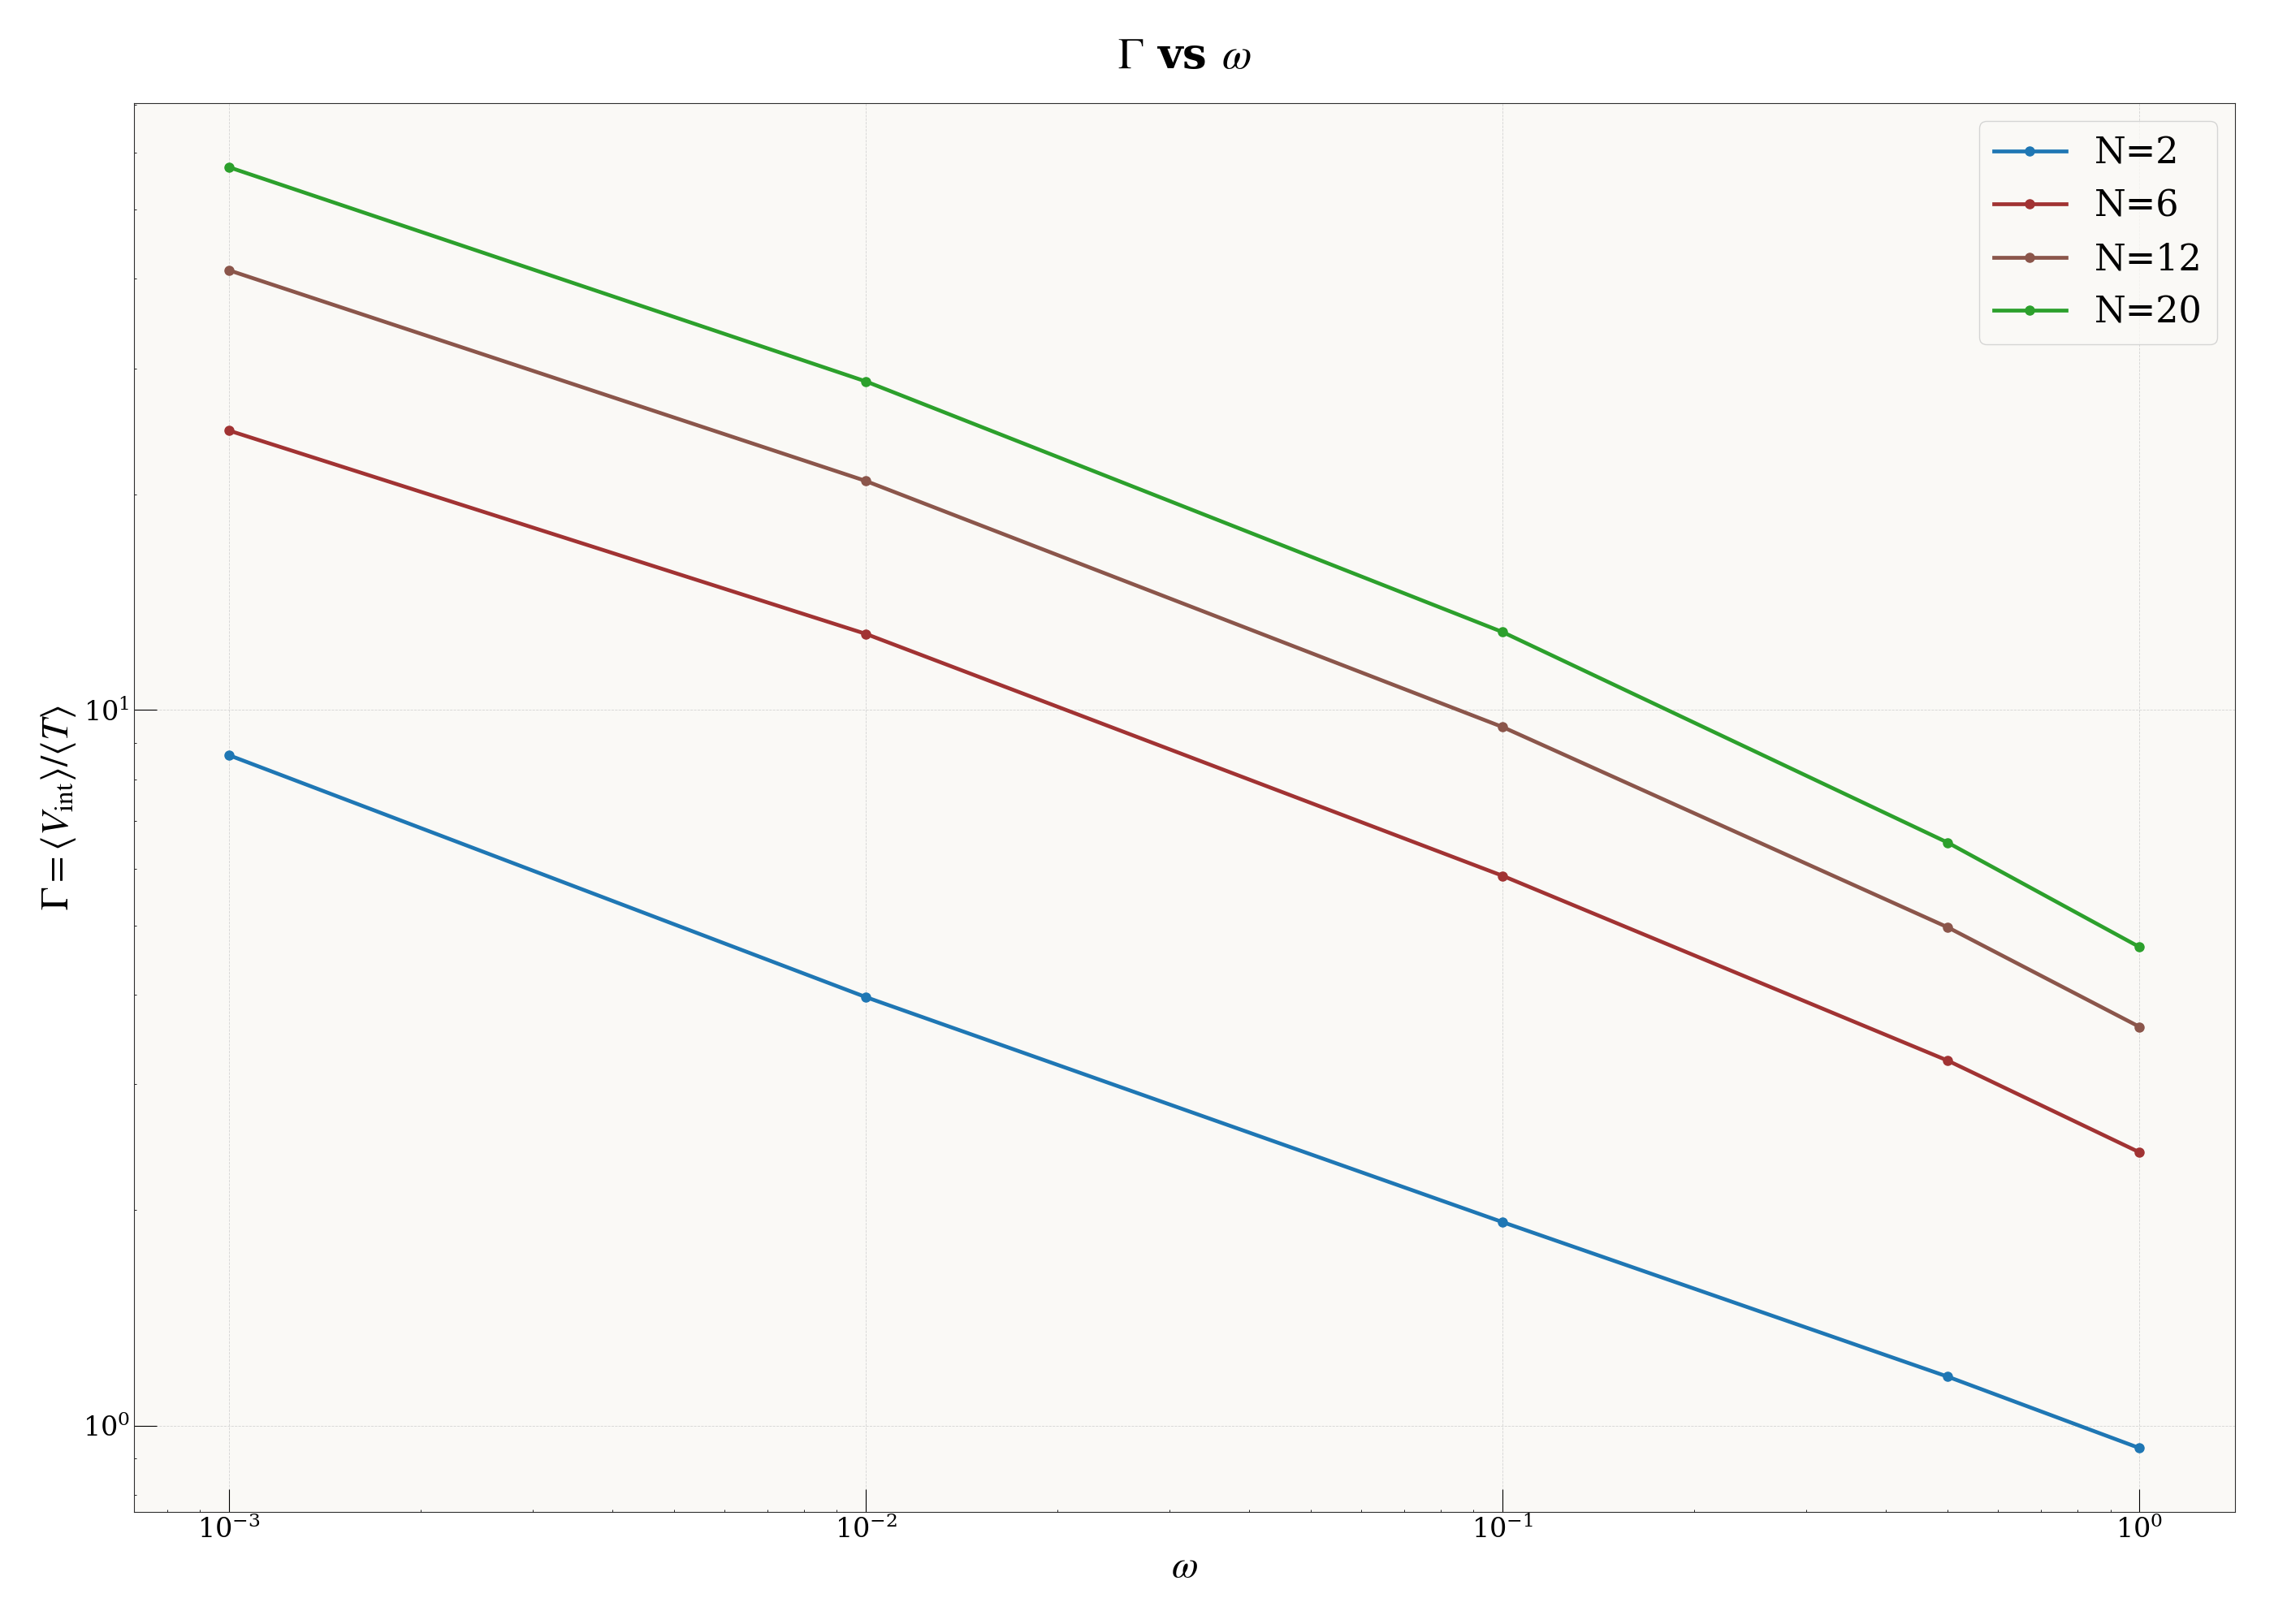
\includegraphics[width=\linewidth]{figures/energy/ratios_allN_Gamma.png}
      \vspace{2pt}
      {\scriptsize (a) $\Gamma(\omega)=\langle V_{\rm int}\rangle/\langle T\rangle$ (log--log). Interaction dominance increases as $\omega\to 0$.}
    \column{0.49\textwidth}
      \centering
      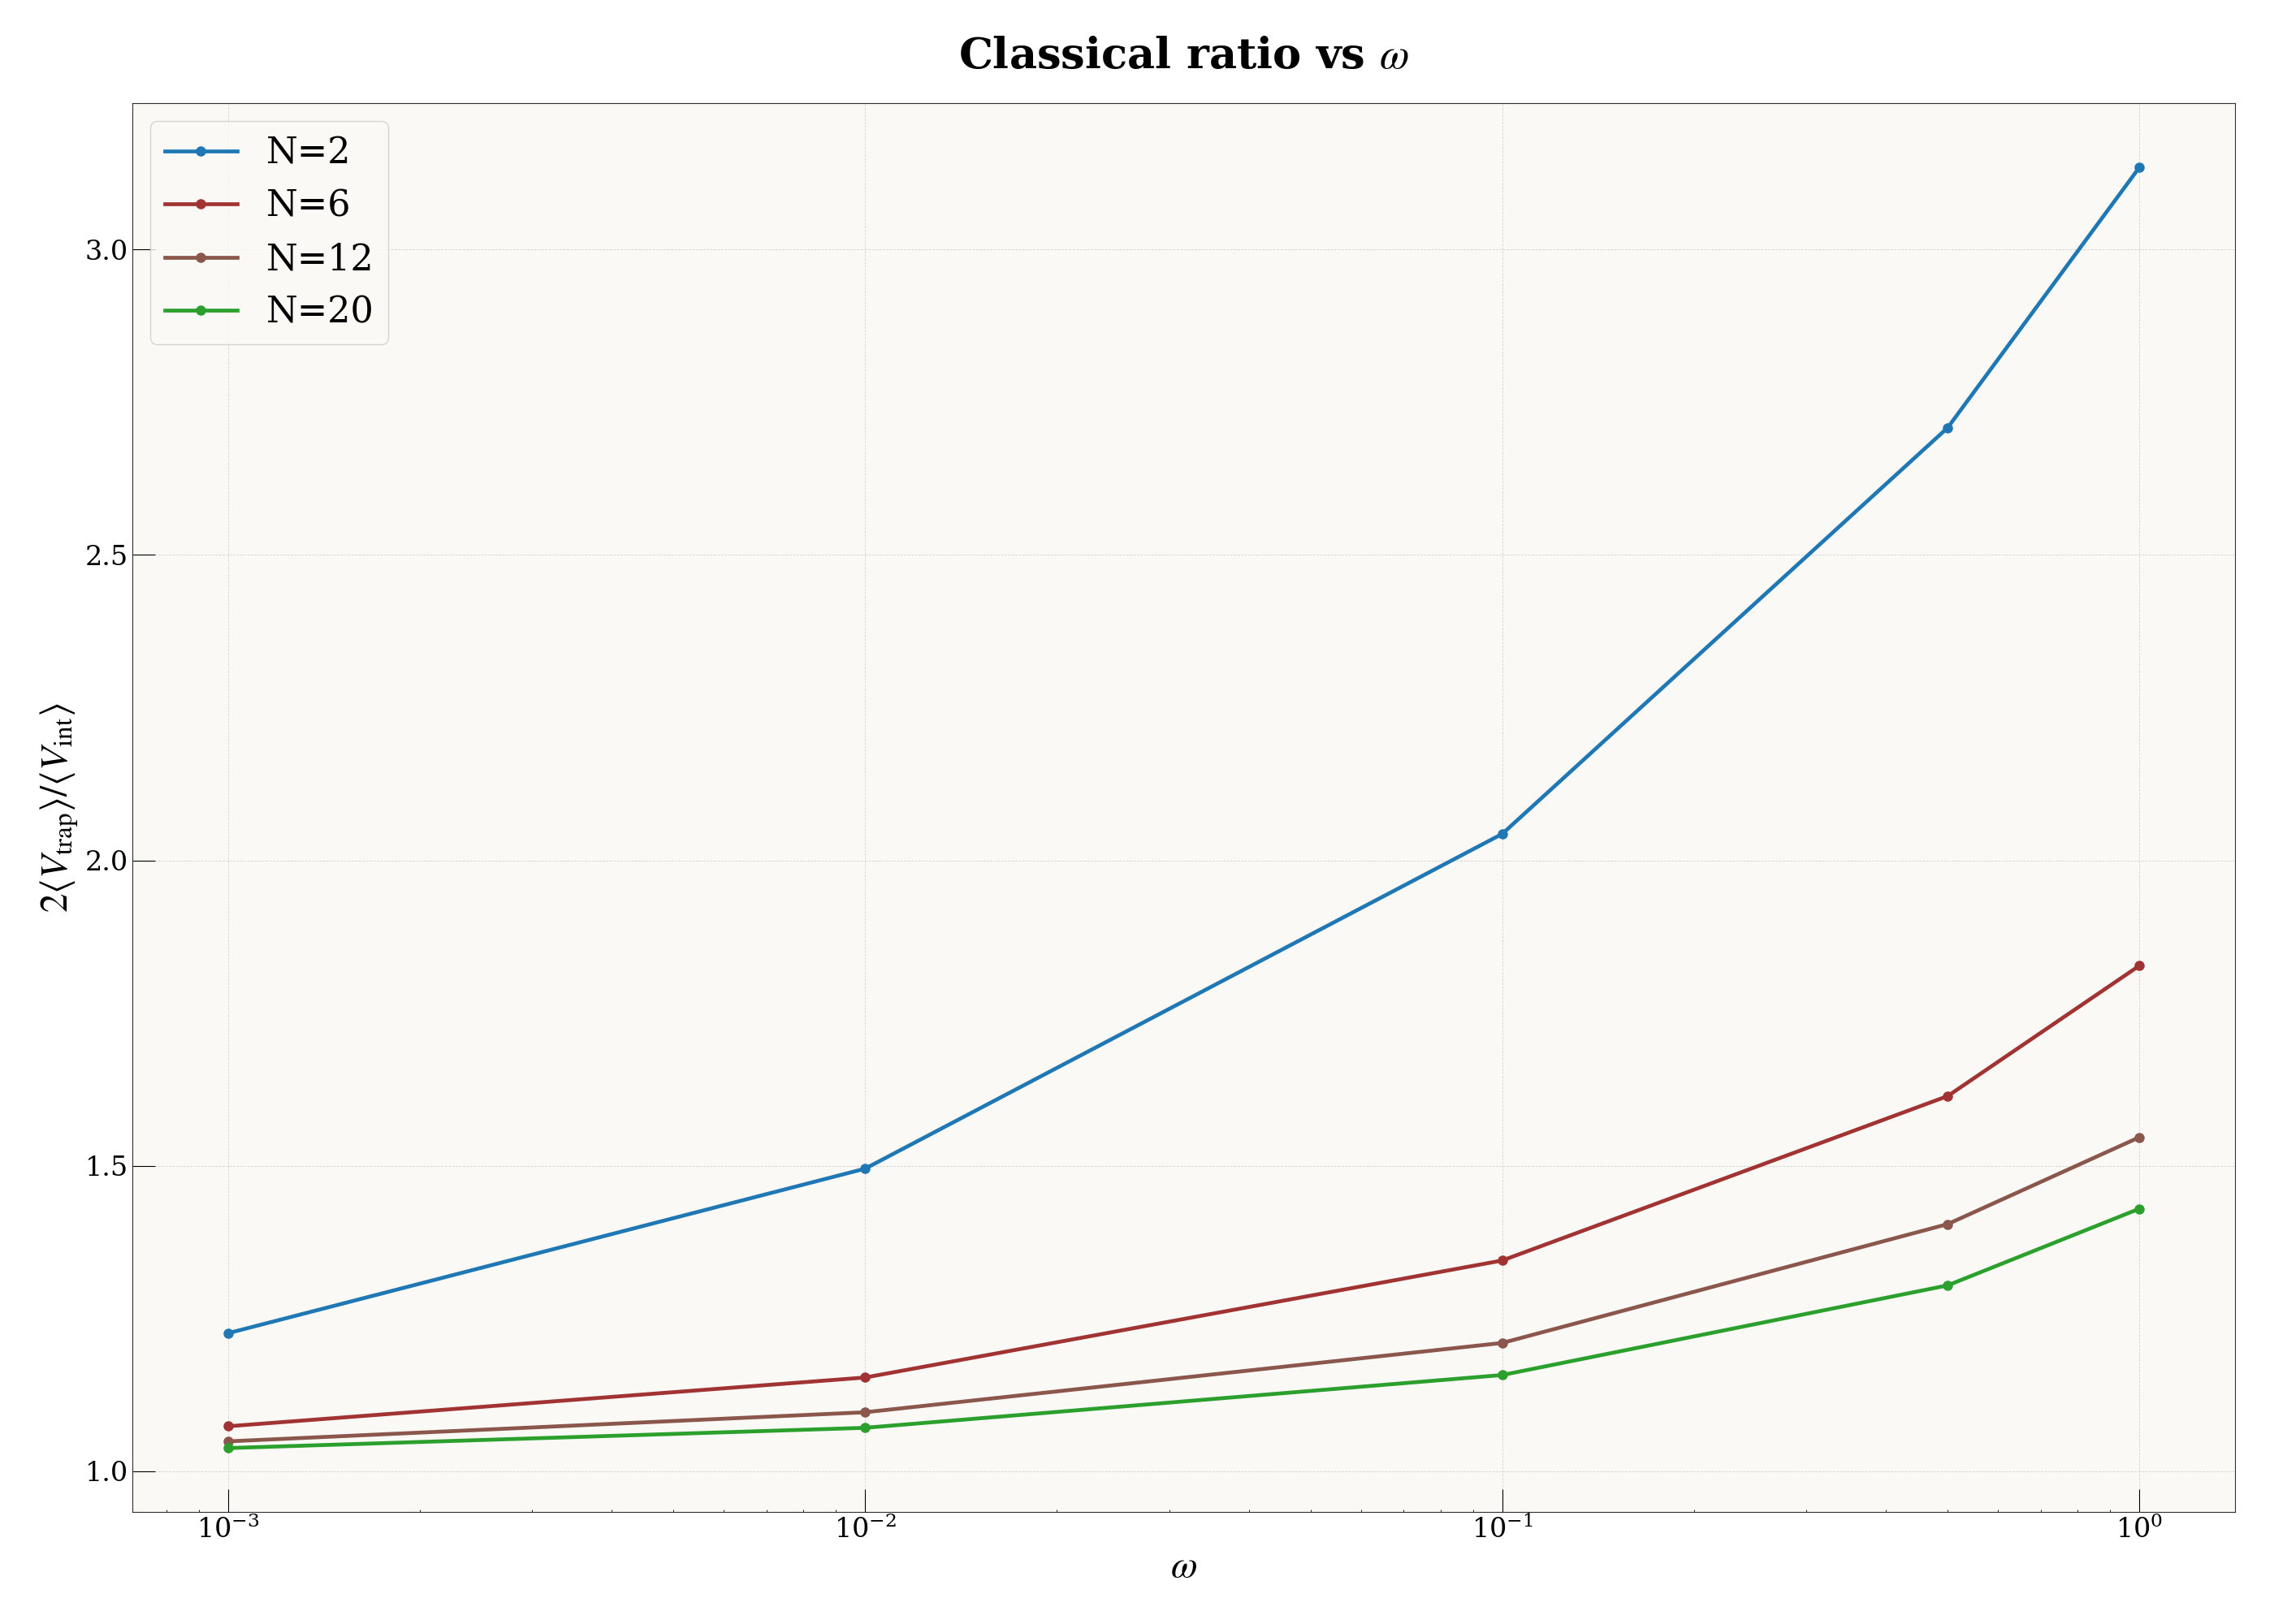
\includegraphics[width=\linewidth]{figures/energy/ratios_allN_classical.png}
      \vspace{2pt}
      {\scriptsize (b) $\mathcal{C}(\omega)=2\langle V_{\rm trap}\rangle/\langle V_{\rm int}\rangle$.}
  \end{columns}

\end{frame}




\begin{frame}{Reproducibility Across Seeds: CI Benchmark ($N=2$--$6$, $\omega=1$)}
  \begin{center}
    \renewcommand{\arraystretch}{1.30}
    \small
    \begin{tabular}{c|c|ccc|cc}
      \toprule
      $N$ & $E_{\rm CI}$ (au) &
      Seed 42 & Seed 314 & Seed 901 &
      Spread (au) & Max $|$err$|$ \\
      \midrule
      2 & 2.254424 &
        2.253853 & 2.254049 & 2.253171 &
        0.00088 & 0.056\% \\
      3 & 3.637002 &
        3.636503 & 3.636209 & 3.636661 &
        0.00029 & 0.022\% \\
      4 & 5.104449 &
        5.103305 & 5.103369 & 5.103568 &
        0.00026 & 0.022\% \\
      6 & 8.217032$^\dagger$ &
        8.213596 & 8.214344 & 8.213966 &
        0.00075 & 0.042\% \\
      \bottomrule
    \end{tabular}
    \normalsize
  \end{center}
  \vspace{0.15cm}
  \small$\dagger$ $N=6$: $n_{\rm sp}=10$, $n_{\rm ci}=500$ (retains 0.05\% of $10^6$ configurations).\normalsize

  \vspace{0.2cm}
  \begin{alertblock}{Key result}
    \textbf{Every single run lies below its CI reference.}
    Non-MCMC training achieves sub-0.06\% accuracy across all $N$,
    with three independent seeds. Seed spread decreases with $N$. Loss functions do not increase.
  \end{alertblock}
\end{frame}


%% ============================================================
\section{Summary and Outlook}
%% ============================================================

%%
\begin{frame}{Summary: Energetics}
  \begin{columns}[T]
    \column{0.50\textwidth}
      \begin{block}{Energetic accuracy}
        \begin{itemize}
          \item Residual pretraining + SR tail pipeline
          \item $N=2$: both PINN+BF and PINN+CTNN agree with DMC
                to within statistical uncertainty
          \item $N=6,12,20$: PINN+CTNN systematically outperforms
                PINN+BF at moderate/strong confinement
          \item Deviations from DMC: $\lesssim 0.05\%$ in benchmarked
                regimes
        \end{itemize}
      \end{block}
    \column{0.50\textwidth}
      \begin{block}{Energy partitioning}
        \begin{itemize}
          \item $\Gamma(\omega)$: interaction-to-kinetic ratio grows
                from $<1$ to $\sim 57$ across the $\omega$ range
          \item $\mathcal{C}(\omega)\to 1$: quasi-classical balance
                at $\omega=10^{-3}$; better approached for larger $N$
          \item $r_{\rm rms}$: $\sim\!70\times$ expansion from
                $\omega=1$ to $\omega=10^{-3}$
        \end{itemize}
      \end{block}
  \end{columns}
\end{frame}


%%
\begin{frame}{Methodological Contributions}
  \begin{enumerate}\itemsep5pt
    \item \textbf{Architecture.}
          Permutation-invariant DeepSets + safe pair features; PINN loss with explicit
          physical constraints.

    \item \textbf{Training pipeline.}
          Residual-based pretraining $\to$ SR tail

  \end{enumerate}

  \vspace{0.3cm}
  \begin{alertblock}{Broader applicability}
    Same PINN framework is directly applicable to:
    other 2D/3D trapped systems $\cdot$ real-time dynamics $\cdot$
    excited states $\cdot$ open quantum systems $\cdot$
    device-level quantum dot modelling.
  \end{alertblock}
\end{frame}

%%
\begin{frame}{PINNs vs.\ VMC: Complementary Strengths}
  \vspace{0.3cm}
  \begin{columns}[T]
    \column{0.48\textwidth}
      \begin{block}{PINN advantages}
        \begin{itemize}
          \item Wave function is a continuous function of coordinates
          \item Natural access to excited states, complex geometries,
                and time-dependent problems
          \item Antisymmetry and normalisation as modular, explicit constraints
        \end{itemize}
      \end{block}
    \column{0.48\textwidth}
      \begin{block}{VMC advantages}
        \begin{itemize}
          \item Established workhorse for large-$N$ ground states
          \item Efficient MC sampling of high-dimensional spaces
          \item Variational upper bounds by construction
          \item Rich library of optimized ansatz forms
        \end{itemize}
      \end{block}
  \end{columns}

  \vspace{0.3cm}
  \begin{alertblock}{Outlook}
    VMC excels at large-$N$ ground states;
    PINNs are strong candidates for continuous-space, dynamical, constrained, and
    few-to-intermediate-body problems.
    Cross-fertilization between the two frameworks is an important direction.
  \end{alertblock}
\end{frame}

%%
\begin{frame}{Open Questions and Future Directions}
  \begin{columns}[T]
    \column{0.50\textwidth}
      \textbf{Computational / methodological}
      \begin{itemize}
        \item Scaling to $N>20$: sparse/message-passing architectures
              to reduce $O(N^2)$ cost, work in progress
        \item Transfer learning: pre-train on one $\omega$, fine-tune
              across the full $\omega$ grid
        \item Excited states: add orthogonality constraints to loss
        \item Real-time dynamics: extend PINN loss with time dependence
        \item Improved optimizers: ?
      \end{itemize}
    \column{0.50\textwidth}
      \textbf{Physics questions}
      \begin{itemize}
        \item Transition to Wigner-Seitz 
        \item Spin degree of freedom and magnetic field effects
        \item Coupled dots and transport / conductance calculations
        \item Entanglement structure of the many-body wave function
        \item Connection to 2D Wigner crystal in the thermodynamic limit
      \end{itemize}
  \end{columns}
\end{frame}

%%
\begin{frame}{Conclusions}
  \begin{enumerate}\itemsep6pt
    \item \textbf{PINNs are accurate} for quantum dots at $N=2$--$20$
          across five orders of magnitude in $\omega$, matching DMC
          benchmarks to $\lesssim 0.05\%$.


    \item \textbf{Energy partitioning and virial validation} confirm
          physical correctness even without DMC references.


    \item \textbf{PINNs provide a unified, physics-grounded framework}
          for few-to-intermediate quantum many-body problems in
          continuous space — with natural extensions to dynamics and
          excited states.
  \end{enumerate}
\end{frame}

\appendix

\begin{frame}{Activation Functions and Higher-Order Derivatives}
      \begin{itemize}
        \item PINNs require second- (or higher-) order derivatives through AD
        \item Activation function choice is critical for $\ell \ge 2$ PDEs
        \item \textbf{Smooth activations required:} $\tanh$, SiLU, Softplus
        \item \textbf{ReLU is unsuitable} for second-order operators
              (second derivative is zero almost everywhere)
      \end{itemize}
\end{frame}


\begin{frame}{Network Architecture}
  \begin{columns}[T]
    \column{0.48\textwidth}
      \begin{block}{Ground-state PINN Jastrow}
        \begin{itemize}
          \item 2 hidden layers, width 64, GELU activations
          \item Input: all pairwise distances + absolute positions
          \item Output: scalar log-amplitude correction $J$
          \item Backflow: optional (2 layers, width 32);
                \alert{disabled} in all production runs
          \item Parameters: ${\sim}25$K ($N=2$) to ${\sim}45$K ($N=6$)
        \end{itemize}
      \end{block}
    \column{0.48\textwidth}
      \begin{block}{Spectral network (imaginary-time evolution)}
        \begin{itemize}
          \item 3 temporal modes $\{A_k(\tau)\}$ + constant
          \item Spatial network: 2 layers, width 32 nodes
          \item Boundary condition: $g \to 0$ as $\tau\to\infty$
                enforced analytically
        \end{itemize}
      \end{block}
      \vspace{0.2cm}
      \begin{alertblock}{Wavefunction form}
        $\psi = \exp(J)\cdot D$ \quad (Jastrow $\times$ Slater determinant)\\[3pt]
        Singlet: $\log|\psi_{\rm singlet}| =
          \mathrm{logaddexp}(J(\mathbf{r}_1,\mathbf{r}_2),\,J(\mathbf{r}_2,\mathbf{r}_1))$
      \end{alertblock}
  \end{columns}
\end{frame}

\begin{frame}{Training Protocol}
      \textbf{Ground-state training (all production runs)}
      \begin{itemize}
        \item Optimizer: Adam, $\text{lr}=10^{-4}$, cosine warm-up
              (200--400 epochs), $\text{lr}_{\rm min}=0.1\times\text{lr}$
        \item Batch size $n_{\rm coll}$: 512 ($N\leq4$), 1024 ($N=6$),
              2048 ($N=8$)
        \item Laplacian: finite difference ($h=0.01$) for $N>4$
        \item Gradient clip: $0.2$
      \end{itemize}
\end{frame}

%%
\begin{frame}{Training Pipeline and Benchmark Strategy}
  \begin{columns}[T]
    \column{0.52\textwidth}
      \textbf{Training pipeline}
      \begin{enumerate}
        \item \textbf{Residual-based pretraining:}
              PINN loss enforces the many-body Schr\"odinger equation
              at collocation points
        \item \textbf{Stochastic Reconfiguration (SR) tail:}
              second-order-like variational refinement; improves energy
              and wave-function quality
      \end{enumerate}
      \vspace{0.3cm}
      \textbf{Internal consistency check}\\
      Harmonic-plus-Coulomb virial identity:
      \[
        2\langle T\rangle = 2\langle V_{\rm trap}\rangle
        - \langle V_{\rm int}\rangle
      \]
      Satisfied to sub-percent accuracy (worst case $\lesssim 0.4\%$).
    \column{0.44\textwidth}
      \begin{block}{Benchmark scope}
        \begin{itemize}
          \item $N=2,6,12,20$ electrons
          \item $\omega\in\{10^{-3},10^{-2},0.1,0.5,1.0\}$
          \item Compared to diffusion Monte Carlo (DMC) where available
          \item Two ans\"atze: PINN+BF and PINN+CTNN
        \end{itemize}
      \end{block}
  \end{columns}
\end{frame}

%% ─── Reproducibility: seed spread vs CI reference ──────────────────────────

%% ─── Implementation details: benchmark reference, architecture, protocol ────
\begin{frame}{Exact Diagonalization Reference}
      \textbf{CI via 2D DVR (discrete variable representation)}
      \begin{enumerate}
        \item Each of $K$ wells contributes $n_{\rm sp}$ single-particle
              orbitals from its local HO basis
        \item $N$-particle product space: $n_{\rm sp}^N$ configurations,
              sorted by non-interacting energy
      \end{enumerate}
      \begin{tabular}{c|ccc|c}
        \toprule
        $N$ & $n_{\rm sp}$ & $n_{\rm ci}$ & grid & SP energy \\
        \midrule
        2--4 & 40  & 300 & $24\!\times\!24$ & 0.998 \\
        6    & 10  & 500 & $24\!\times\!16$ & 1.000 \\
        \bottomrule
      \end{tabular}
\end{frame}


\end{document}





